\documentclass[spanish,]{article}
\usepackage{lmodern}
\usepackage{amssymb,amsmath}
\usepackage{ifxetex,ifluatex}
\usepackage{fixltx2e} % provides \textsubscript
\ifnum 0\ifxetex 1\fi\ifluatex 1\fi=0 % if pdftex
  \usepackage[T1]{fontenc}
  \usepackage[utf8]{inputenc}
\else % if luatex or xelatex
  \ifxetex
    \usepackage{mathspec}
  \else
    \usepackage{fontspec}
  \fi
  \defaultfontfeatures{Ligatures=TeX,Scale=MatchLowercase}
\fi
% use upquote if available, for straight quotes in verbatim environments
\IfFileExists{upquote.sty}{\usepackage{upquote}}{}
% use microtype if available
\IfFileExists{microtype.sty}{%
\usepackage{microtype}
\UseMicrotypeSet[protrusion]{basicmath} % disable protrusion for tt fonts
}{}
\usepackage[margin=1in]{geometry}
\usepackage{hyperref}
\hypersetup{unicode=true,
            pdfauthor={Alejandro Campoy Nieves; Gema Correa Fernández; Luis Gallego Quero; Jonathan Martín Valera; Andrea Morales Garzón},
            pdfborder={0 0 0},
            breaklinks=true}
\urlstyle{same}  % don't use monospace font for urls
\ifnum 0\ifxetex 1\fi\ifluatex 1\fi=0 % if pdftex
  \usepackage[shorthands=off,main=spanish]{babel}
\else
  \usepackage{polyglossia}
  \setmainlanguage[]{spanish}
\fi
\usepackage{color}
\usepackage{fancyvrb}
\newcommand{\VerbBar}{|}
\newcommand{\VERB}{\Verb[commandchars=\\\{\}]}
\DefineVerbatimEnvironment{Highlighting}{Verbatim}{commandchars=\\\{\}}
% Add ',fontsize=\small' for more characters per line
\usepackage{framed}
\definecolor{shadecolor}{RGB}{248,248,248}
\newenvironment{Shaded}{\begin{snugshade}}{\end{snugshade}}
\newcommand{\KeywordTok}[1]{\textcolor[rgb]{0.13,0.29,0.53}{\textbf{#1}}}
\newcommand{\DataTypeTok}[1]{\textcolor[rgb]{0.13,0.29,0.53}{#1}}
\newcommand{\DecValTok}[1]{\textcolor[rgb]{0.00,0.00,0.81}{#1}}
\newcommand{\BaseNTok}[1]{\textcolor[rgb]{0.00,0.00,0.81}{#1}}
\newcommand{\FloatTok}[1]{\textcolor[rgb]{0.00,0.00,0.81}{#1}}
\newcommand{\ConstantTok}[1]{\textcolor[rgb]{0.00,0.00,0.00}{#1}}
\newcommand{\CharTok}[1]{\textcolor[rgb]{0.31,0.60,0.02}{#1}}
\newcommand{\SpecialCharTok}[1]{\textcolor[rgb]{0.00,0.00,0.00}{#1}}
\newcommand{\StringTok}[1]{\textcolor[rgb]{0.31,0.60,0.02}{#1}}
\newcommand{\VerbatimStringTok}[1]{\textcolor[rgb]{0.31,0.60,0.02}{#1}}
\newcommand{\SpecialStringTok}[1]{\textcolor[rgb]{0.31,0.60,0.02}{#1}}
\newcommand{\ImportTok}[1]{#1}
\newcommand{\CommentTok}[1]{\textcolor[rgb]{0.56,0.35,0.01}{\textit{#1}}}
\newcommand{\DocumentationTok}[1]{\textcolor[rgb]{0.56,0.35,0.01}{\textbf{\textit{#1}}}}
\newcommand{\AnnotationTok}[1]{\textcolor[rgb]{0.56,0.35,0.01}{\textbf{\textit{#1}}}}
\newcommand{\CommentVarTok}[1]{\textcolor[rgb]{0.56,0.35,0.01}{\textbf{\textit{#1}}}}
\newcommand{\OtherTok}[1]{\textcolor[rgb]{0.56,0.35,0.01}{#1}}
\newcommand{\FunctionTok}[1]{\textcolor[rgb]{0.00,0.00,0.00}{#1}}
\newcommand{\VariableTok}[1]{\textcolor[rgb]{0.00,0.00,0.00}{#1}}
\newcommand{\ControlFlowTok}[1]{\textcolor[rgb]{0.13,0.29,0.53}{\textbf{#1}}}
\newcommand{\OperatorTok}[1]{\textcolor[rgb]{0.81,0.36,0.00}{\textbf{#1}}}
\newcommand{\BuiltInTok}[1]{#1}
\newcommand{\ExtensionTok}[1]{#1}
\newcommand{\PreprocessorTok}[1]{\textcolor[rgb]{0.56,0.35,0.01}{\textit{#1}}}
\newcommand{\AttributeTok}[1]{\textcolor[rgb]{0.77,0.63,0.00}{#1}}
\newcommand{\RegionMarkerTok}[1]{#1}
\newcommand{\InformationTok}[1]{\textcolor[rgb]{0.56,0.35,0.01}{\textbf{\textit{#1}}}}
\newcommand{\WarningTok}[1]{\textcolor[rgb]{0.56,0.35,0.01}{\textbf{\textit{#1}}}}
\newcommand{\AlertTok}[1]{\textcolor[rgb]{0.94,0.16,0.16}{#1}}
\newcommand{\ErrorTok}[1]{\textcolor[rgb]{0.64,0.00,0.00}{\textbf{#1}}}
\newcommand{\NormalTok}[1]{#1}
\usepackage{graphicx,grffile}
\makeatletter
\def\maxwidth{\ifdim\Gin@nat@width>\linewidth\linewidth\else\Gin@nat@width\fi}
\def\maxheight{\ifdim\Gin@nat@height>\textheight\textheight\else\Gin@nat@height\fi}
\makeatother
% Scale images if necessary, so that they will not overflow the page
% margins by default, and it is still possible to overwrite the defaults
% using explicit options in \includegraphics[width, height, ...]{}
\setkeys{Gin}{width=\maxwidth,height=\maxheight,keepaspectratio}
\IfFileExists{parskip.sty}{%
\usepackage{parskip}
}{% else
\setlength{\parindent}{0pt}
\setlength{\parskip}{6pt plus 2pt minus 1pt}
}
\setlength{\emergencystretch}{3em}  % prevent overfull lines
\providecommand{\tightlist}{%
  \setlength{\itemsep}{0pt}\setlength{\parskip}{0pt}}
\setcounter{secnumdepth}{0}
% Redefines (sub)paragraphs to behave more like sections
\ifx\paragraph\undefined\else
\let\oldparagraph\paragraph
\renewcommand{\paragraph}[1]{\oldparagraph{#1}\mbox{}}
\fi
\ifx\subparagraph\undefined\else
\let\oldsubparagraph\subparagraph
\renewcommand{\subparagraph}[1]{\oldsubparagraph{#1}\mbox{}}
\fi

%%% Use protect on footnotes to avoid problems with footnotes in titles
\let\rmarkdownfootnote\footnote%
\def\footnote{\protect\rmarkdownfootnote}

%%% Change title format to be more compact
\usepackage{titling}

% Create subtitle command for use in maketitle
\newcommand{\subtitle}[1]{
  \posttitle{
    \begin{center}\large#1\end{center}
    }
}

\setlength{\droptitle}{-2em}

  \title{}
    \pretitle{\vspace{\droptitle}}
  \posttitle{}
    \author{Alejandro Campoy Nieves \\ Gema Correa Fernández \\ Luis Gallego Quero \\ Jonathan Martín Valera \\ Andrea Morales Garzón}
    \preauthor{\centering\large\emph}
  \postauthor{\par}
      \predate{\centering\large\emph}
  \postdate{\par}
    \date{14 de noviembre de 2018}

\usepackage{fancyhdr}
\fancyfoot[CO,CE]{My footer}
\usepackage{color}
\usepackage{colortbl}
\usepackage{multicol}
\usepackage{multirow}

\begin{document}

\thispagestyle{empty}

\begin{center} \huge \textbf{Tratamiento Inteligente de datos} \end{center}

\vspace{0.3cm}

\begin{center} \huge \textbf{(TID)} \end{center}

\vspace{1.7cm}

\begin{center} \Large \textbf{\textsc{Prácticas de la asignatura}} \end{center}

\vspace{0.2cm}

\begin{center} \large \textbf{2018-2019} \end{center}

\vspace{2.5cm}

\textbf{\large En colaboración con:} \vspace{0.2cm}

\begin{figure}[h]
    \centering
    
\includegraphics[width=0.7\textwidth]{imagenes/logoUGR.jpg}
    \label{imagen2}
\end{figure}

\vspace{2.5cm}

\hspace{8.5cm}{\large \textbf{Participantes}}

\vspace{0.25cm}

\hspace{8.5cm}{Alejandro Campoy Nieves:  \href{mailto:alejandroac79@correo.ugr.es}{\textcolor{blue}{\underline{alejandroac79@correo.ugr.es}}}}

\vspace{0.15cm}

\hspace{8.5cm}{Gema Correa Fernández:  \href{mailto:gecorrea@correo.ugr.es}{\textcolor{blue}{\underline{gecorrea@correo.ugr.es}}} }

\vspace{0.15cm}

\hspace{8.5cm}{Luis Gallego Quero:  \href{mailto:lgaq94@correo.ugr.es}{\textcolor{blue}{\underline{lgaq94@correo.ugr.es}}} }

\vspace{0.15cm}

\hspace{8.5cm}{Jonathan Martín Valera:  \href{mailto:jmv742@correo.ugr.es}{\textcolor{blue}{\underline{jmv742@correo.ugr.es}}} }

\vspace{0.15cm}

\hspace{8.5cm}{Andrea Morales Garzón:  \href{mailto:andreamgmg@correo.ugr.es}{\textcolor{blue}{\underline{andreamgmg@correo.ugr.es}}} }

\vspace{0.15cm}

\newpage

\thispagestyle{empty} \tableofcontents
\newpage

\thispagestyle{empty} \listoffigures
\newpage

\thispagestyle{empty} \listoftables
\newpage

\pagestyle{fancy} \fancyhf{}
\lhead{Proyecto: Técnicas aplicadas para análisis inteligente de datos}
\rhead{\thepage} \setcounter{page}{1}

\section{Descripción de los paquetes
necesarios}\label{descripcion-de-los-paquetes-necesarios}

A continuación, se describen los paquetes necesarios para el desarollo
del proyecto:

\begin{itemize}
\item
  \href{https://cran.r-project.org/web/packages/tm/tm.pdf}{\texttt{tm}}
  : Paquete específico para minería de datos, permite procesar datos de
  tipo texto. Se puede instalar usando :
  \emph{install.packages(``tm'')}.
\item
  \href{https://cran.r-project.org/web/packages/SnowballC/SnowballC.pdf}{\texttt{SnowballC}}
  : Paquete adicional para minería de datos, implementa un algoritmo que
  permite reducir el número de términos con lo que trabajar, es decir,
  agrupa aquellos términos que contienen la misma raíz. El paquete
  soporta los siguientes idiomas: alemán, danés, español, finlandés,
  francés, húngaro, inglés, italiano, noruego, portugués, rumano, ruso,
  sueco y turco. Se puede instalar usando :
  \emph{install.packages(``SnowballC'')}.
\item
  \href{https://cran.r-project.org/web/packages/wordcloud/wordcloud.pdf}{\texttt{wordcloud}}
  : Paquete para crear gráficas de nubes de palabras, permitiendo
  visualizar las diferencias y similitudes entre documentos. Se puede
  instalar usando : \emph{install.packages(``wordcloud'')}.
\item
  \href{https://cran.r-project.org/web/packages/arules/arules.pdf}{\texttt{arules}}
  : Paquete que proporciona la infraestructura para representar,
  manipular y analizar datos y patrones de transacción (conjuntos de
  elementos frecuentes y reglas de asociación). Se puede instalar usando
  : \emph{install.packages(``arules'')}.
\item
  \href{https://cran.r-project.org/web/packages/arulesViz/arulesViz.pdf}{\texttt{arulesViz}}
  : Paquete que extiende el paquete `arules' con varias técnicas de
  visualización para reglas de asociación y conjuntos de elementos. El
  paquete también incluye varias visualizaciones interactivas para la
  exploración de reglas. Se puede instalar usando :
  \emph{install.packages(``arulesViz'')}.
\item
  \href{https://cran.r-project.org/web/packages/devtools/devtools.pdf}{\texttt{devtools}}
  : Paquete que contiene una colección de herramientas de desarrollo de
  paquetes, usando conjuntamento con \texttt{rword2vec}, para obtener la
  agrupación de sinónimos. Se puede instalar usando :
  \emph{install.packages(``devtools'')}.
\item
  \href{https://github.com/mukul13/rword2vec}{\texttt{rword2vec}} :
  Paquete que toma un corpus de texto como entrada y produce los
  vectores de palabra como salida, usado especialmente para obtener las
  distancias que existen entre un término y los términos semejantes en
  el texto de formación (aprende la representación vectorial de las
  palabras). Se puede instalar usando :
  \emph{install\_github(``mukul13/rword2vec'')}.
\end{itemize}

\newpage

\section{1. Comprender el problema a
resolver}\label{comprender-el-problema-a-resolver}

El \emph{dataset}
\href{https://archive.ics.uci.edu/ml/datasets/Drug+Review+Dataset+\%28Druglib.com\%29}{\textbf{Drug
Review Dataset}}, proporcionado por
\href{https://archive.ics.uci.edu/ml/index.php}{\emph{UCI Machine
Learning Repository}}, contiene una exhaustiva base de datos de
medicamentos específicos, en la cual, el conjunto de datos muestra
revisiones de pacientes sobre medicamentos específicos para unas
condiciones particulares. Dichas revisiones se encuentran desglosadas en
función del tema que se esté tratando: beneficios, efectos secundarios y
comentarios generales. De igual modo, se dispone de una calificación de
satisfacción general, es decir, de una calificación en base a los
efectos secundarios del medicamento y de otra en base a la efectividad
del mismo.

En este proyecto nos centraremos en el \textbf{análisis y experiencia
qué tienen los usuarios con ciertos tipos de medicamentos}, para la
realización y aplicación de las técnicas explicadas a lo largo del
curso. Para ello, se proponen los siguientes objetivos principales:

\begin{itemize}
\item
  Realizar un análisis de sentimientos a partir de la experiencia de
  dichos usuarios en el uso de ciertos medicamentos, como por ejemplo
  ver la efectividad del medicamento cuánto está relacionado con los
  efectos secundarios o beneficios del mismo.
\item
  Compatibilizar dicho modelo de datos con otros conjuntos de datos
  aportados en \href{https://www.drugs.com/}{\textbf{Drugs.com}}.
\end{itemize}

Las características de este conjunto de datos vienen descritas en la
siguiente tabla \ref{tabla:preseleccion}:

\begin{table}[h]
    \begin{center}
        \begin{tabular}{|>{\columncolor[rgb]{0.94,0.97,1.0}}l|c|}
            \hline 
            \textbf{Características del Data Set} & Multivariable, texto \\ \hline
            \textbf{Características de los atributos} & Entero \\ \hline
            \textbf{Tareas asociadas} & Clasificación, regresión, clustering \\ \hline
            \textbf{Número de instancias} & 4143 \\ \hline
            \textbf{Número de atributos} & 8 \\ \hline
            \textbf{Valores vacíos} & N/A \\ \hline
            \textbf{Área} & N/A \\ \hline
            \textbf{Fecha de donación} & 10/02/2018 \\ \hline
            \textbf{Veces visualizado} & 11047 \\ \hline
        \end{tabular}
        \caption{Información del conjunto de datos}
        \label{tabla:preseleccion}
    \end{center}
\end{table}

Los datos se dividen en un conjunto train (75\%) y otro conjunto test
(25\%) y se almacenan en dos archivos \emph{.tsv}
(tab-separated-values), respectivamente. Los atributos que tenemos en
este dataset son:

\begin{enumerate}
\def\labelenumi{\arabic{enumi}.}
\tightlist
\item
  \textbf{urlDrugName} (categorical): nombre del medicamento/fármaco
\item
  \textbf{rating} (numerical): clasificación o puntuación del 1 a 10 del
  medicamento según el paciente
\item
  \textbf{effectiveness} (categorical): clasificación de la efectividad
  del medicamento según el paciente (5 posibles valores)
\item
  \textbf{sideEffects} (categorical): clasificación de los efectos
  secundarios del medicamento según el paciente (5 posibles valores)
\item
  \textbf{condition} (categorical): nombre de la condición (diagnóstico)
\item
  \textbf{benefitsReview} (text): opinión del paciente sobre los
  beneficios
\item
  \textbf{sideEffectsReview} (text): opinión del paciente sobre los
  efectos secundarios
\item
  \textbf{commentsReview} (text): comentario general del paciente
\end{enumerate}

\section{2. Preprocesamiento de datos}\label{preprocesamiento-de-datos}

En este apartado, pondremos los datos a punto para la aplicación de
diversas técnicas. Por tanto, para poder analizar dicho \emph{dataset} y
realizar el preprocesamiento al mismo, lo primero que se va hacer es
leer el conjunto de datos \emph{train} y \emph{test}.

\subsection{2.1. Lectura de datos}\label{lectura-de-datos}

A continuación, mediante la función \texttt{read.table} procedemos a la
lectura de los datos:

\subsubsection{2.1.1. Lectura de datos
train}\label{lectura-de-datos-train}

Se va a procedeer a la lectura del conjunto de datos de entrenamiento.

\begin{Shaded}
\begin{Highlighting}[]
\CommentTok{# Lectura de datos train}
\NormalTok{datos_train <-}\StringTok{ }\KeywordTok{read.table}\NormalTok{(}\StringTok{"datos/drugLibTrain_raw.tsv"}\NormalTok{, }\DataTypeTok{sep=}\StringTok{"}\CharTok{\textbackslash{}t}\StringTok{"}\NormalTok{, }\DataTypeTok{comment.char=}\StringTok{""}\NormalTok{,}
                          \DataTypeTok{quote =} \StringTok{"}\CharTok{\textbackslash{}"}\StringTok{"}\NormalTok{, }\DataTypeTok{header=}\OtherTok{TRUE}\NormalTok{)}
\end{Highlighting}
\end{Shaded}

Disponemos una matriz de 3107 filas x 9 columnas, asimismo vamos a ver
un ejemplo de como distribuida la información, en donde para la fila
tercera encontramos la siguiente información:

\begin{table}[h]
  \centering
    \begin{tabular}{|l|l|l|l|l|l|l|l|l|}
      \hline
      \rowcolor[rgb]{0.94,0.97,1.0} \textbf{X} & \textbf{urlDrugName} & \textbf{rating} & \textbf{effectiveness} 
      & \textbf{sideEffects} &\textbf{condition} \\ \hline
      1146 & ponstel & 10 & Highly Effective & No Side Effects & menstrual cramps  \\ \hline
    \end{tabular}
  \caption{Información contenida en una fila del conjunto de entrenamiento I}
  \label{tabla:datos_trainI}
\end{table}

\begin{table}[h]
  \centering
    \begin{tabular}{|m{5cm}|m{3cm}|m{7cm}|}
      \hline
      \rowcolor[rgb]{0.94,0.97,1.0} \textbf{benefitsReview} & \textbf{sideEffectsReview} & \textbf{commentsReview} \\ \hline
      I was used to having cramps so badly that they would leave me balled up in bed for at least 2 days. The Ponstel doesn't take the pain away completely, but takes the edge off so much that normal activities were possible. Definitely a miracle medication!! & Heavier bleeding and clotting than normal. & I took 2 pills at the onset of my menstrual cramps and then every 8-12 hours took 1 pill as needed for about 3-4 days until cramps were over. If cramps are bad, make sure to take every 8 hours on the dot because the medication stops working suddenly and unfortunately takes about an hour to an hour and a half to kick back in.. if cramps are only moderate, taking every 12 hours is okay. \\ \hline
    \end{tabular}
  \caption{Información contenida en una fila del conjunto de entrenamiento II}
  \label{tabla:datos_trainII}
\end{table}

De las tablas \ref{tabla:datos_trainI} y \ref{tabla:datos_trainII}
podemos extraer que el medicamento \textbf{ponstel} con identificador
\textbf{1146}, tiene la máxima puntuación por parte del paciente
(\textbf{rating = 10}), el cual tiene un alto nivel de efectividad
(\textbf{Highly Effective}) sin efectos secundarios
(\textbf{No Side Effects}), usado para dolores menstruales
(\textbf{menstrual cramps}), en donde el paciente dice que de estar
tumbado en la cama con dolores ha pasado a poder realizar las
actividades sin ningún impedimento. Además, asegura que tomar este
medicamento le ha supuesto un sangrado más abundante y coagulación de lo
normal. La dosis del medicamento oscila entre una píldora cada 8-12
horas durante 3-4 días.

\subsubsection{2.1.2. Lectura de datos
test}\label{lectura-de-datos-test}

Se va a procedeer a la lectura del conjunto de datos de prueba.

\begin{Shaded}
\begin{Highlighting}[]
\CommentTok{# Lectura de datos test}
\NormalTok{datos_test <-}\StringTok{ }\KeywordTok{read.table}\NormalTok{(}\StringTok{"./datos/drugLibTest_raw.tsv"}\NormalTok{, }\DataTypeTok{sep=}\StringTok{"}\CharTok{\textbackslash{}t}\StringTok{"}\NormalTok{, }\DataTypeTok{comment.char=}\StringTok{""}\NormalTok{,}
                         \DataTypeTok{quote =} \StringTok{"}\CharTok{\textbackslash{}"}\StringTok{"}\NormalTok{, }\DataTypeTok{header=}\OtherTok{TRUE}\NormalTok{)}
\end{Highlighting}
\end{Shaded}

Disponemos una matriz de 1036 filas x 9 columnas, asimismo vamos a ver
un ejemplo de como distribuida la información, en donde para la fila
primera encontramos la siguiente información:

De las tablas \ref{tabla:datos_testI} y \ref{tabla:datos_testII} podemos
extraer que el medicamento \textbf{biaxin} con identificador
\textbf{1366}, tiene una puntuación de 9 por parte del paciente
(\textbf{rating = 9}), el cual tiene un nive considerable de efectividad
(\textbf{Considerably Effective}) con efectos secundarios leves
(\textbf{Mild Side Effects}), usado para la infección sinusal
(\textbf{sinus infection}), en donde el paciente dice que no está muy
seguro de si el antibiótico ha destruido las bacterias que causan su
infección sinusal. Además, asegura que tomar este medicamento le da algo
de dolor de espalda y algunas náuseas. El paciente tomó los antibióticos
durante 14 días y la infección sinusal desapareció al sexto día.

\begin{table}[h]
  \centering
    \begin{tabular}{|l|l|l|l|l|l|l|l|l|}
      \hline
      \rowcolor[rgb]{0.94,0.97,1.0} \textbf{X} & \textbf{urlDrugName} & \textbf{rating} & \textbf{effectiveness} 
      & \textbf{sideEffects} &\textbf{condition} \\ \hline
      1366 & biaxin & 9 & Considerably Effective & Mild Side Effects & sinus infection  \\ \hline
    \end{tabular}
  \caption{Información contenida en una fila del conjunto de prueba I}
  \label{tabla:datos_testI}
\end{table}

\begin{table}[h]
  \centering
    \begin{tabular}{|m{7cm}|m{3cm}|m{5cm}|}
      \hline
      \rowcolor[rgb]{0.94,0.97,1.0} \textbf{benefitsReview} & \textbf{sideEffectsReview} & \textbf{commentsReview} \\ \hline
      The antibiotic may have destroyed bacteria causing my sinus infection. But it may also have been caused by a virus, so its hard to say. & Some back pain, some nauseau. & Took the antibiotics for 14 days. Sinus infection was gone after the 6th day. \\ \hline
    \end{tabular}
  \caption{Información contenida en una fila del conjunto de prueba II}
  \label{tabla:datos_testII}
\end{table}

La representación del documento se llevará a cabo utilizando palabras,
después de un debido filtrado para minimizar la dimensión del espacio de
trabajo.

\subsection{2.2. Procesamiento de los
datos}\label{procesamiento-de-los-datos}

Dado que la representación total del documento puede tener una alta
dimensión, se va a procedeer a construir un corpus, necesario para la
aplicación de métodos de limpieza y esructuración del texto de entrada e
identificación de un subconjunto simplificado de las características del
documento con el fin de poder ser representado en un análisis posterior.

\subsubsection{2.2.1. Eliminar columnas}\label{eliminar-columnas}

El primer paso que vamos a realizar es la \textbf{eliminación de
columnas}, las cuales contienen información irrelevante para nuestro
análisis.

\paragraph{Eliminar columna ID}\label{eliminar-columna-id}

Al conjunto de datos utilizado se le ha añadido de forma automática una
novena columna, que representa un ID para cada uno de los datos con los
que estamos trabajando. Como este ID no nos aporta información alguna,
hemos decidido quitarla directamente del \emph{dataframe}. Esta columna
se corresponde con la primera columna, por lo cuál, debemos eliminar la
columna que se corresponde con la posición 1. Los cambios que hacemos en
el \emph{dataset} deben modificarse tanto en el conjunto de test como el
de train, para que los resultados sean consistentes.

\begin{Shaded}
\begin{Highlighting}[]
\NormalTok{datos_train =}\StringTok{ }\NormalTok{datos_train[}\OperatorTok{-}\DecValTok{1}\NormalTok{] }\CommentTok{# Eliminar columna para el ID en el train}
\NormalTok{datos_test =}\StringTok{ }\NormalTok{datos_test[}\OperatorTok{-}\DecValTok{1}\NormalTok{] }\CommentTok{# Eliminar columna para el ID en el test}
\end{Highlighting}
\end{Shaded}

\paragraph{Eliminar columna de
commentsReview}\label{eliminar-columna-de-commentsreview}

Consideramos que la información contenida en \emph{commentsReview} no es
de nuestro interés. En este atributo se almacena texto, en el cual los
consumidores de los medicamentos suelen poner en la mayoría de casos la
frecuencia o la dosis con la que consumen la misma. En otros casos menos
frecuentes, se establecen comentarios más arbitrarios en el que se
muestran sus sensaciones o información sin relevancia. Incluso en
algunos casos este campo aparece vacío. Es por eso, que hemos decidido
eliminar la columna, tanto para el conjunto test como el train.

\begin{Shaded}
\begin{Highlighting}[]
\NormalTok{datos_train =}\StringTok{ }\NormalTok{datos_train[}\OperatorTok{-}\DecValTok{8}\NormalTok{] }\CommentTok{# Eliminar columna para el commentsReview en el train}
\NormalTok{datos_test =}\StringTok{ }\NormalTok{datos_test[}\OperatorTok{-}\DecValTok{8}\NormalTok{] }\CommentTok{# Eliminar columna para el commentsReview en el test}
\end{Highlighting}
\end{Shaded}

\subsubsection{2.2.2. Categorización de
variables}\label{categorizacion-de-variables}

Para poder analizar y trabajar más fácilmente con la información de
\emph{sideEffects} y \emph{effectiveness}, se va a realizar una
conversión de dichas columnas a forma cuantitativa, es decir, vamos
asignar una etiqueta numérica a cada valor pertinente, tanto para para
\emph{train} como \emph{test}.

A continuación, vamos a cuantificar la columna de \emph{sideEffects},
para ello se añade una nueva columna a nuestro conjunto de datos
denominada \emph{sideEffectsNumber} que nos clasifica los posibles
valores de la columna \emph{sideEffects} en un rango numérico,
comprendido entre 1 y 5. Dicha columna hace referencia a la
clasificación de los efectos secundarios del medicamento según el
paciente, en donde la etiqueta con valor 1 hará referencia a que no haya
ningún efecto secundario y la etiqueta con valor 5 a que tiene efectos
secundarios extremadamente graves:

\begin{itemize}
\tightlist
\item
  Extremely Severe Side Effects (efectos secundarios extremadamente
  graves) : 5
\item
  Severe Side Effects (efectos secundarios graves): 4
\item
  Moderate Side Effects (efectos secundarios moderados) : 3
\item
  Mild Side Effects (efectos secundarios leves) : 2
\item
  No Side Effects (sin efectos secundarios) : 1
\end{itemize}

\begin{Shaded}
\begin{Highlighting}[]
\CommentTok{# Datos Train}
\NormalTok{datos_train}\OperatorTok{$}\NormalTok{sideEffectsNumber[datos_train}\OperatorTok{$}\NormalTok{sideEffects}\OperatorTok{==}\StringTok{"Extremely Severe Side Effects"}\NormalTok{]<-}\DecValTok{5}
\NormalTok{datos_train}\OperatorTok{$}\NormalTok{sideEffectsNumber[datos_train}\OperatorTok{$}\NormalTok{sideEffects}\OperatorTok{==}\StringTok{"Severe Side Effects"}\NormalTok{]<-}\DecValTok{4}
\NormalTok{datos_train}\OperatorTok{$}\NormalTok{sideEffectsNumber[datos_train}\OperatorTok{$}\NormalTok{sideEffects}\OperatorTok{==}\StringTok{"Moderate Side Effects"}\NormalTok{] <-}\StringTok{ }\DecValTok{3}
\NormalTok{datos_train}\OperatorTok{$}\NormalTok{sideEffectsNumber[datos_train}\OperatorTok{$}\NormalTok{sideEffects}\OperatorTok{==}\StringTok{"Mild Side Effects"}\NormalTok{]<-}\StringTok{ }\DecValTok{2}
\NormalTok{datos_train}\OperatorTok{$}\NormalTok{sideEffectsNumber[datos_train}\OperatorTok{$}\NormalTok{sideEffects}\OperatorTok{==}\StringTok{"No Side Effects"}\NormalTok{]<-}\StringTok{ }\DecValTok{1}

\CommentTok{# Datos Test}
\NormalTok{datos_test}\OperatorTok{$}\NormalTok{sideEffectsNumber[datos_test}\OperatorTok{$}\NormalTok{sideEffects}\OperatorTok{==}\StringTok{"Extremely Severe Side Effects"}\NormalTok{]<-}\DecValTok{5}
\NormalTok{datos_test}\OperatorTok{$}\NormalTok{sideEffectsNumber[datos_test}\OperatorTok{$}\NormalTok{sideEffects}\OperatorTok{==}\StringTok{"Severe Side Effects"}\NormalTok{]<-}\DecValTok{4}
\NormalTok{datos_test}\OperatorTok{$}\NormalTok{sideEffectsNumber[datos_test}\OperatorTok{$}\NormalTok{sideEffects}\OperatorTok{==}\StringTok{"Moderate Side Effects"}\NormalTok{]<-}\DecValTok{3}
\NormalTok{datos_test}\OperatorTok{$}\NormalTok{sideEffectsNumber[datos_test}\OperatorTok{$}\NormalTok{sideEffects}\OperatorTok{==}\StringTok{"Mild Side Effects"}\NormalTok{]<-}\DecValTok{2}
\NormalTok{datos_test}\OperatorTok{$}\NormalTok{sideEffectsNumber[datos_test}\OperatorTok{$}\NormalTok{sideEffects}\OperatorTok{==}\StringTok{"No Side Effects"}\NormalTok{]<-}\DecValTok{1}
\end{Highlighting}
\end{Shaded}

Podemos comprobar que se ha creado la nueva columna
\emph{sideEffectsNumber}, y que se han añadido los cambios comentados
anteriormente.

\begin{Shaded}
\begin{Highlighting}[]
\KeywordTok{head}\NormalTok{(datos_train}\OperatorTok{$}\NormalTok{sideEffectsNumber, }\DecValTok{10}\NormalTok{) }
\end{Highlighting}
\end{Shaded}

\begin{verbatim}
##  [1] 2 4 1 2 4 4 2 1 1 5
\end{verbatim}

Volvemos a aplicar el mismo procedimiento para la columna de
\emph{effectiveness}, creándonos para ello una columna denominada
\emph{effectivenessNumber}. Dicha columna, hace referencia a la
clasificación de la efectividad del medicamento según el paciente, en
donde la etiqueta con valor 1 hace referencia a que el medicamente es
ineficaz y la etiqueta con valor 5 a que el medicamente es altamente
eficaz:

\begin{itemize}
\tightlist
\item
  Highly Effective (altamente efectivo): 5
\item
  Considerably Effective (considerablemente efectivo) : 4
\item
  Moderately Effective (moderadamente efectivo) : 3
\item
  Marginally Effective (marginalmente efectivo) : 2
\item
  Ineffective (ineficaz) : 1
\end{itemize}

\begin{Shaded}
\begin{Highlighting}[]
\CommentTok{# Datos de entrenamiento}
\NormalTok{datos_train}\OperatorTok{$}\NormalTok{effectivenessNumber[datos_train}\OperatorTok{$}\NormalTok{effectiveness}\OperatorTok{==}\StringTok{"Highly Effective"}\NormalTok{]<-}\DecValTok{5}
\NormalTok{datos_train}\OperatorTok{$}\NormalTok{effectivenessNumber[datos_train}\OperatorTok{$}\NormalTok{effectiveness}\OperatorTok{==}\StringTok{"Considerably Effective"}\NormalTok{]<-}\DecValTok{4}
\NormalTok{datos_train}\OperatorTok{$}\NormalTok{effectivenessNumber[datos_train}\OperatorTok{$}\NormalTok{effectiveness}\OperatorTok{==}\StringTok{"Moderately Effective"}\NormalTok{]<-}\DecValTok{3}
\NormalTok{datos_train}\OperatorTok{$}\NormalTok{effectivenessNumber[datos_train}\OperatorTok{$}\NormalTok{effectiveness}\OperatorTok{==}\StringTok{"Marginally Effective"}\NormalTok{]<-}\DecValTok{2}
\NormalTok{datos_train}\OperatorTok{$}\NormalTok{effectivenessNumber[datos_train}\OperatorTok{$}\NormalTok{effectiveness}\OperatorTok{==}\StringTok{"Ineffective"}\NormalTok{]<-}\StringTok{ }\DecValTok{1}

\CommentTok{# Datos de test}
\NormalTok{datos_test}\OperatorTok{$}\NormalTok{effectivenessNumber[datos_test}\OperatorTok{$}\NormalTok{effectiveness}\OperatorTok{==}\StringTok{"Highly Effective"}\NormalTok{]<-}\DecValTok{5}
\NormalTok{datos_test}\OperatorTok{$}\NormalTok{effectivenessNumber[datos_test}\OperatorTok{$}\NormalTok{effectiveness}\OperatorTok{==}\StringTok{"Considerably Effective"}\NormalTok{]<-}\DecValTok{4}
\NormalTok{datos_test}\OperatorTok{$}\NormalTok{effectivenessNumber[datos_test}\OperatorTok{$}\NormalTok{effectiveness}\OperatorTok{==}\StringTok{"Moderately Effective"}\NormalTok{]<-}\DecValTok{3}
\NormalTok{datos_test}\OperatorTok{$}\NormalTok{effectivenessNumber[datos_test}\OperatorTok{$}\NormalTok{effectiveness}\OperatorTok{==}\StringTok{"Marginally Effective"}\NormalTok{]<-}\DecValTok{2}
\NormalTok{datos_test}\OperatorTok{$}\NormalTok{effectivenessNumber[datos_test}\OperatorTok{$}\NormalTok{effectiveness}\OperatorTok{==}\StringTok{"Ineffective"}\NormalTok{]<-}\DecValTok{1}
\end{Highlighting}
\end{Shaded}

Comprobamos que se ha creado la nueva columna
\emph{effectivenessNumber}, y que se han añadido los nuevos cambios.

\begin{Shaded}
\begin{Highlighting}[]
\KeywordTok{head}\NormalTok{(datos_train}\OperatorTok{$}\NormalTok{effectivenessNumber, }\DecValTok{10}\NormalTok{) }
\end{Highlighting}
\end{Shaded}

\begin{verbatim}
##  [1] 5 5 5 2 2 1 5 4 5 1
\end{verbatim}

Por tanto, una vez eliminadas las columnas anteriores y modificadas las
necesarias, ya podemos continuar con el procesamiento de los datos. Para
ello, lo primero tenemos que hacer es cargar la librería que procesa los
datos de tipo texto en R, para la construcción y manipulación del
corpus. La librería más conocida se llama \textbf{tm}, aunque también
haremos uso del paquete \textbf{SnowballC} para realizar el
\emph{Stemming}. Si no tenemos instaladas las librerías:

\begin{Shaded}
\begin{Highlighting}[]
\CommentTok{# Paquete para minería de datos, permite procesar datos de tipo texto}
\CommentTok{# El paquete tm, necesita el paquete NLP}
\KeywordTok{library}\NormalTok{(}\StringTok{"NLP"}\NormalTok{)}
\KeywordTok{library}\NormalTok{(}\StringTok{"tm"}\NormalTok{)}

\CommentTok{# Paquete para minería de datos, agrupa aquellos términos que contienen la misma raíz}
\KeywordTok{library}\NormalTok{(}\StringTok{"SnowballC"}\NormalTok{)}
\end{Highlighting}
\end{Shaded}

\subsubsection{2.2.3. Creación del corpus}\label{creacion-del-corpus}

Para poder obtener la estructura con la que vamos a procesar nuestra
información, debemos obtener un vector con documentos. En nuestro caso,
cada uno de los documentos se corresponde con una opinión sobre un
fármaco (\emph{benefitsReview}) y los efectos que tiene
(\emph{sideEffectsReview}). Para ello, primero debemos de construir un
vector con todas los opiniones del \emph{dataframe} y convertir cada
elemento del vector al formato de documento. Podemos usar la función
\emph{VectorSource} para hacer esta conversión. Se deberán realizar
todas las modificaciones tanto para el conjunto train como test.

\begin{Shaded}
\begin{Highlighting}[]
\CommentTok{# Datos train}

\CommentTok{# Nos quedamos con la única columna del dataset que nos interesa. }
\CommentTok{# Necesitamos obtenerla en forma de vector, y no como un dataframe de una columna, }
\CommentTok{# por lo que usamos as.vector para hacer la conversión}
\NormalTok{benefits_train_review_data =}\StringTok{ }\KeywordTok{as.vector}\NormalTok{(datos_train}\OperatorTok{$}\NormalTok{benefitsReview)}
\NormalTok{effects_train_review_data =}\StringTok{ }\KeywordTok{as.vector}\NormalTok{(datos_train}\OperatorTok{$}\NormalTok{sideEffectsReview)}

\CommentTok{# Lo convertimos en la estructura de documento, y lo guardamos ya en el corpus }
\CommentTok{# que lo vamos a utilizar}
\NormalTok{benefits_train_corpus =}\StringTok{ }\NormalTok{(}\KeywordTok{VectorSource}\NormalTok{(benefits_train_review_data))}
\NormalTok{effects_train_corpus =}\StringTok{ }\NormalTok{(}\KeywordTok{VectorSource}\NormalTok{(effects_train_review_data))}

\CommentTok{# Creamos el propio corpus}
\NormalTok{benefits_train_corpus <-}\StringTok{ }\KeywordTok{Corpus}\NormalTok{(benefits_train_corpus)}
\NormalTok{effects_train_corpus <-}\StringTok{ }\KeywordTok{Corpus}\NormalTok{(effects_train_corpus)}
\end{Highlighting}
\end{Shaded}

\begin{Shaded}
\begin{Highlighting}[]
\CommentTok{# Datos test}

\CommentTok{# Nos quedamos con la única columna del dataset que nos interesa. }
\CommentTok{# Necesitamos obtenerla en forma de vector, y no como un dataframe de una columna, }
\CommentTok{# por lo que usamos as.vector para hacer la conversión}
\NormalTok{benefits_test_review_data =}\StringTok{ }\KeywordTok{as.vector}\NormalTok{(datos_test}\OperatorTok{$}\NormalTok{benefitsReview)}
\NormalTok{effects_test_review_data =}\StringTok{ }\KeywordTok{as.vector}\NormalTok{(datos_test}\OperatorTok{$}\NormalTok{sideEffectsReview)}

\CommentTok{# Lo convertimos en la estructura de documento, y lo guardamos ya en el corpus }
\CommentTok{# que lo vamos a utilizar}
\NormalTok{benefits_test_corpus =}\StringTok{ }\NormalTok{(}\KeywordTok{VectorSource}\NormalTok{(benefits_test_review_data))}
\NormalTok{effects_test_corpus =}\StringTok{ }\NormalTok{(}\KeywordTok{VectorSource}\NormalTok{(effects_test_review_data))}

\CommentTok{# Creamos el propio corpus}
\NormalTok{benefits_test_corpus <-}\StringTok{ }\KeywordTok{Corpus}\NormalTok{(benefits_test_corpus)}
\NormalTok{effects_test_corpus <-}\StringTok{ }\KeywordTok{Corpus}\NormalTok{(effects_test_corpus)}
\end{Highlighting}
\end{Shaded}

Podemos ver que funciona accediendo a uno cualquiera, de la forma
\texttt{inspect(benefits\_train\_corpus{[}4{]})}:

\begin{figure}[h]
    \centering
    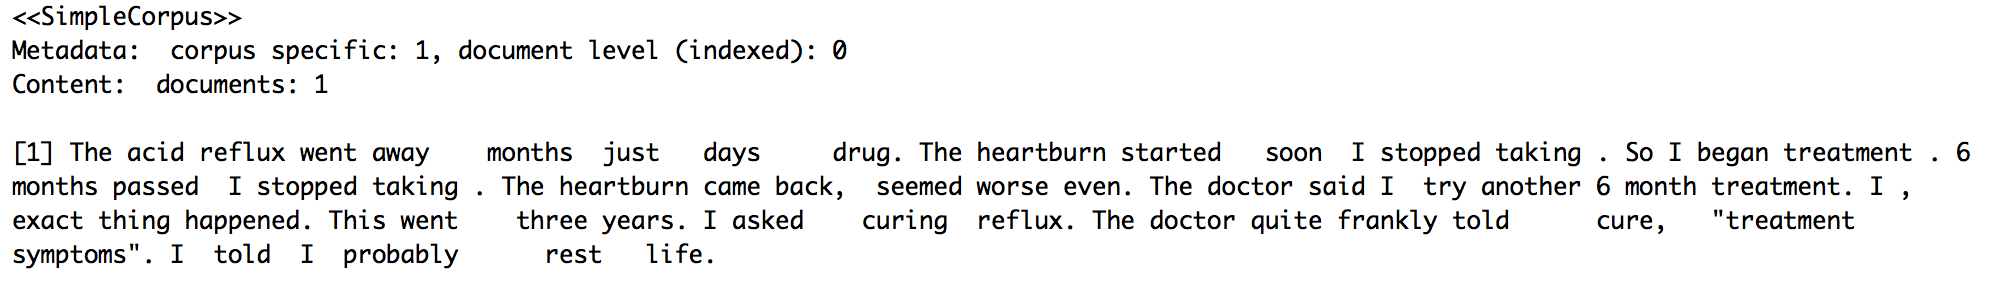
\includegraphics[width=1\textwidth]{imagenes/benefits_train_corpus1.png}
    \caption{Contenido de benefits\_train\_corpus}
    \label{benefits1}
\end{figure}

O de la forma \texttt{benefits\_train\_corpus{[}{[}4{]}{]}\$content}:

\begin{figure}[h]
    \centering
    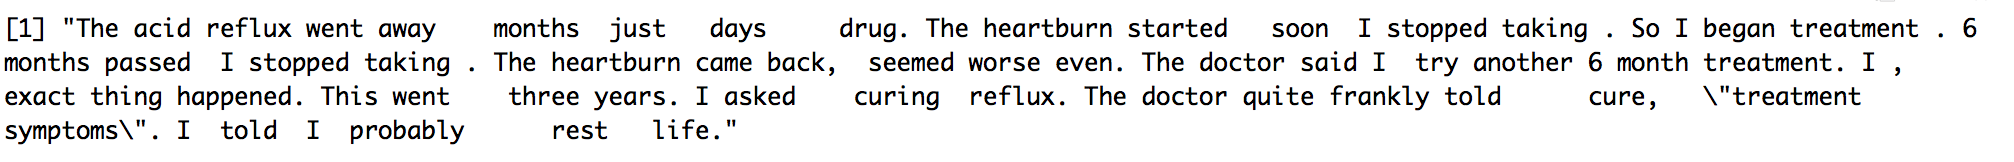
\includegraphics[width=1\textwidth]{imagenes/benefits_train_corpus2.png}
    \caption{Contenido de benefits\_train\_corpus}
    \label{benefits2}
\end{figure}

Y si nos fijamos en el contenido, vemos que tiene signos de puntuación y
exclamación.

\subsubsection{2.2.4. Eliminar signos de
puntuación}\label{eliminar-signos-de-puntuacion}

Como hemos podido ver en el documento que se ha mostrado por pantalla,
en él se aprecia el uso de signos de puntuación y exclamación. En un
principio, no tiene sentido en \textit{Data Mining} contemplar los
signos de puntuación, ya que no nos van a aportar información. Por ello,
los quitamos, como se puede ver a continuación. Con
\texttt{tm\_map(corpus,\ removePunctuation)}, se eliminan los símbolos:
! " \$ \% \& `() * + , - . / : ; \textless{} = \textgreater{} ? @ {[}
~{]} \^{} \_' \{ \textbar{} \} \textasciitilde{}

\begin{Shaded}
\begin{Highlighting}[]
\CommentTok{# Una vez que tenemos el corpus creado, continuamos con el procesamiento para los datos train}
\NormalTok{benefits_train_corpus <-}\StringTok{ }\KeywordTok{tm_map}\NormalTok{(benefits_train_corpus, }\KeywordTok{content_transformer}\NormalTok{(removePunctuation))}
\NormalTok{effects_train_corpus <-}\StringTok{ }\KeywordTok{tm_map}\NormalTok{(effects_train_corpus, }\KeywordTok{content_transformer}\NormalTok{(removePunctuation))}

\CommentTok{# Una vez que tenemos el corpus creado, continuamos con el procesamiento para los datos test}
\NormalTok{benefits_test_corpus <-}\StringTok{ }\KeywordTok{tm_map}\NormalTok{(benefits_test_corpus, }\KeywordTok{content_transformer}\NormalTok{(removePunctuation))}
\NormalTok{effects_test_corpus <-}\StringTok{ }\KeywordTok{tm_map}\NormalTok{(effects_test_corpus, }\KeywordTok{content_transformer}\NormalTok{(removePunctuation))}
\end{Highlighting}
\end{Shaded}

Si volvemos a mostrar la opinión número cuatro, vemos como todos los
signos han desaparecido. De hecho, podemos inspeccionar el corpus, y se
ve como todos los signos de puntuación, exclamación y derivados ya no
están.

\begin{figure}[h]
    \centering
    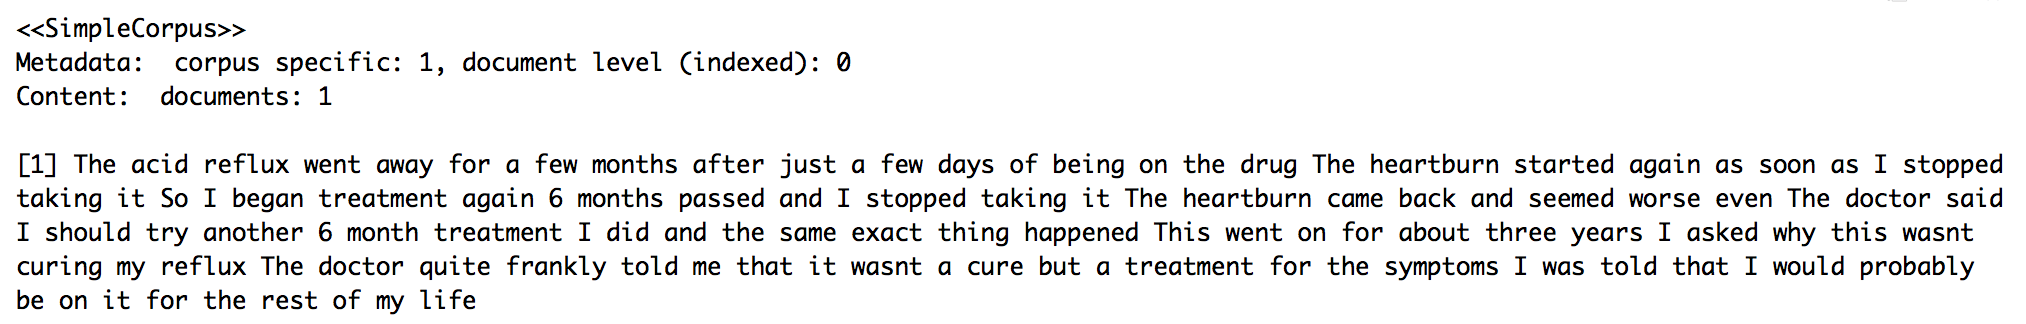
\includegraphics[width=1\textwidth]{imagenes/benefits_signos_puntuacion.png}
    \caption{Contenido de benefits\_train\_corpus con inspect(benefits\_train\_corpus[4])}
    \label{benefits2}
\end{figure}

Ocurre lo mismo con el comentario de efectos número siete.

\begin{figure}[h]
    \centering
    
\includegraphics[width=1\textwidth]{imagenes/effects_signos_puntuacion.png}
    \caption{Contenido de effects\_train\_corpus con inspect(effects\_train\_corpus[7])}
    \label{benefits2}
\end{figure}

\subsubsection{2.2.5. Conversión de las mayúsculas en
minúsculas}\label{conversion-de-las-mayusculas-en-minusculas}

Para poder hacer uso de los términos por igual, debemos convertir las
mayúsculas en minúsculas. Ya que normalmente se convierte en minúsculas
todas las letras para que los comienzos de oración no sean tratados de
manera diferente por los algoritmos.

\begin{Shaded}
\begin{Highlighting}[]
\NormalTok{benefits_train_corpus <-}\StringTok{ }\KeywordTok{tm_map}\NormalTok{(benefits_train_corpus, }\KeywordTok{content_transformer}\NormalTok{(tolower))}
\CommentTok{#inspect(benefits_train_corpus[4])}

\NormalTok{effects_train_corpus <-}\StringTok{ }\KeywordTok{tm_map}\NormalTok{(effects_train_corpus, }\KeywordTok{content_transformer}\NormalTok{(tolower))}
\CommentTok{#inspect(effects_train_corpus[7])}

\NormalTok{benefits_test_corpus <-}\StringTok{ }\KeywordTok{tm_map}\NormalTok{(benefits_test_corpus, }\KeywordTok{content_transformer}\NormalTok{(tolower))}
\NormalTok{effects_test_corpus <-}\StringTok{ }\KeywordTok{tm_map}\NormalTok{(effects_test_corpus, }\KeywordTok{content_transformer}\NormalTok{(tolower))}
\end{Highlighting}
\end{Shaded}

\begin{figure}[h]
    \centering
    
\includegraphics[width=1\textwidth]{imagenes/benefits_mayusculas.png}
    \caption{inspect(benefits\_train\_corpus[4])}
    \label{benefits2}
\end{figure}

\begin{figure}[h]
    \centering
    
\includegraphics[width=1\textwidth]{imagenes/effects_mayusculas.png}
    \caption{inspect(effects\_train\_corpus[7])}
    \label{benefits2}
\end{figure}

\subsubsection{2.2.6. Eliminación de
Stopwords}\label{eliminacion-de-stopwords}

En cualquier idioma, hay palabras que son tan comunes o muy utilizadas
que no aportan información relevante, a dichas palabras se las conoce
como \emph{stopwords} o palabras \emph{stop}. Por ejemplo, en español,
las palabras ``la'', ``a'', ``en'', ``de'' son ejemplos de
\emph{stopwords}. Este tipo de palabras debemos de suprimirlas de
nuestro corpus. Como, en nuestro caso, el contenido del corpus está en
inglés, debemos especificar el idioma correcto para que nos elimine del
corpus las palabras adecuadas en dicho idioma.

\begin{Shaded}
\begin{Highlighting}[]
\NormalTok{benefits_train_corpus <-}\StringTok{ }\KeywordTok{tm_map}\NormalTok{(benefits_train_corpus, }\KeywordTok{content_transformer}\NormalTok{(removeWords), }\KeywordTok{stopwords}\NormalTok{(}\StringTok{"english"}\NormalTok{))}
\CommentTok{#inspect(benefits_train_corpus[4])}

\NormalTok{effects_train_corpus <-}\StringTok{ }\KeywordTok{tm_map}\NormalTok{(effects_train_corpus, }\KeywordTok{content_transformer}\NormalTok{(removeWords), }\KeywordTok{stopwords}\NormalTok{(}\StringTok{"english"}\NormalTok{))}
\KeywordTok{inspect}\NormalTok{(effects_train_corpus[}\DecValTok{7}\NormalTok{])}
\end{Highlighting}
\end{Shaded}

\begin{verbatim}
## <<SimpleCorpus>>
## Metadata:  corpus specific: 1, document level (indexed): 0
## Content:  documents: 1
## 
## [1]   experiences  nausiea heavy moodswings   days    take  decreased appetite   negative affect   shortterm memory
\end{verbatim}

\begin{Shaded}
\begin{Highlighting}[]
\NormalTok{benefits_test_corpus <-}\StringTok{ }\KeywordTok{tm_map}\NormalTok{(benefits_test_corpus, }\KeywordTok{content_transformer}\NormalTok{(removeWords), }\KeywordTok{stopwords}\NormalTok{(}\StringTok{"english"}\NormalTok{))}
\NormalTok{effects_test_corpus <-}\StringTok{ }\KeywordTok{tm_map}\NormalTok{(effects_test_corpus, }\KeywordTok{content_transformer}\NormalTok{(removeWords), }\KeywordTok{stopwords}\NormalTok{(}\StringTok{"english"}\NormalTok{))}
\end{Highlighting}
\end{Shaded}

\begin{figure}[h]
    \centering
    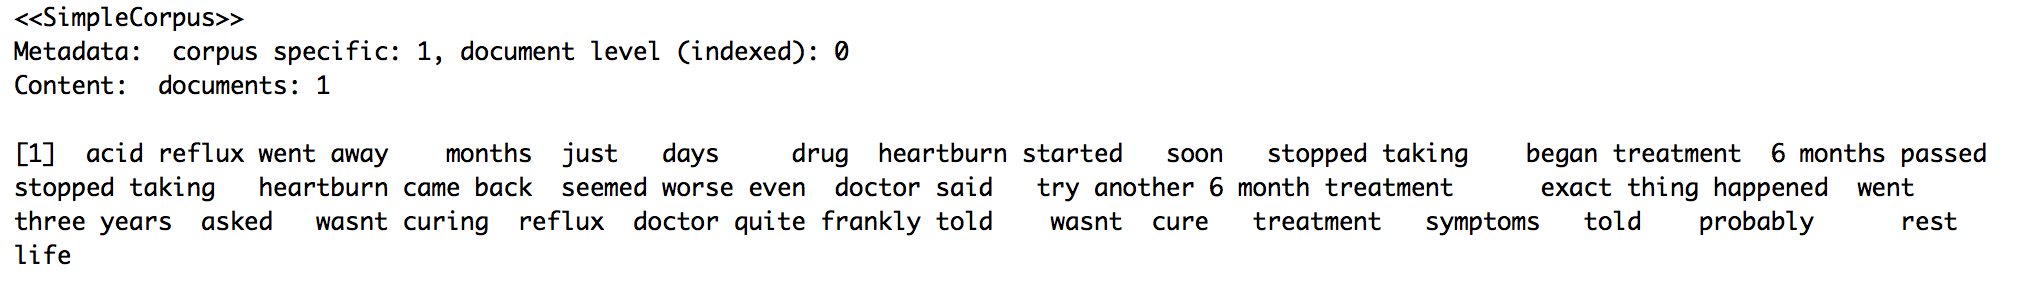
\includegraphics[width=1\textwidth]{imagenes/benefits_stopwords.png}
    \caption{inspect(benefits\_train\_corpus[4])}
    \label{benefits2}
\end{figure}

\begin{figure}[h]
    \centering
    
\includegraphics[width=1\textwidth]{imagenes/effects_stopwords.png}
    \caption{inspect(effects\_train\_corpus[7])}
    \label{benefits2}
\end{figure}

Ahora ya hemos eliminado las stopwords de forma correcta.

\subsubsection{2.2.7. Agrupación de
sinónimos:}\label{agrupacion-de-sinonimos}

Con el fin de disminuir la dimensión del espacio a trabajar, se pueden
identificar palabras distintas con el mismo significado y reemplazarlas
por una sola palabra. Para ello se toman los sinónimos de dicha palabra.
Dentro de las librerías que podemos usar para agrupar sinónimos,
destacamos dos: \texttt{wordnet} y \texttt{rword2vec}. Sin embargo, por
su sencillez se va hacer uso de \texttt{rword2vec}. Previamente, se
obtendrán que palabras son las que mayor frecuencia presentan en nuestro
texto, para ello nos quedamos con las 100 más representativas tanto para
\emph{benefitsReview} como \emph{sideEffectsReview} del conjunto train y
test:

\begin{Shaded}
\begin{Highlighting}[]
\CommentTok{# Columna benefitsReview del conjunto train}

\CommentTok{# Obtenemos su matriz de términos}
\NormalTok{matrix_train_benefits_corpus <-}\StringTok{ }\KeywordTok{TermDocumentMatrix}\NormalTok{(benefits_train_corpus)}
\CommentTok{# No tenemos los datos en la matriz que buscamos, sino en un vector}
\CommentTok{# por tanto, lo convertimos en matriz}
\NormalTok{matrix_train_benefits_corpus <-}\StringTok{ }\KeywordTok{as.matrix}\NormalTok{(matrix_train_benefits_corpus)}
\CommentTok{# Sumamos las filas para obtener la frecuencia de una palabra en benefitsReview}
\NormalTok{matrix_train_benefits_corpus <-}\StringTok{ }\KeywordTok{rowSums}\NormalTok{(matrix_train_benefits_corpus)}
\CommentTok{# Ordenamos de mayor a menor los términos y nos quedamos con lso 100 primeros}
\NormalTok{terms_frecuency_benefits_train_corpus <-}\StringTok{ }\KeywordTok{sort}\NormalTok{(matrix_train_benefits_corpus, }\DataTypeTok{decreasing =} \OtherTok{TRUE}\NormalTok{)}
\NormalTok{terms_frecuency_benefits_train_corpus_}\DecValTok{200}\NormalTok{ <-}\StringTok{ }\NormalTok{terms_frecuency_benefits_train_corpus[}\DecValTok{1}\OperatorTok{:}\DecValTok{200}\NormalTok{]}
\NormalTok{terms_frecuency_benefits_train_corpus_}\DecValTok{200}
\end{Highlighting}
\end{Shaded}

\begin{verbatim}
##          pain        taking          drug          also           day 
##           590           468           438           394           377 
##          skin         sleep     treatment          able    medication 
##           355           348           339           339           333 
##          time        better       effects          take          much 
##           332           326           314           299           289 
##          feel           get      symptoms    depression        helped 
##           280           279           278           278           276 
##          less          side         years       reduced      benefits 
##           269           268           259           256           254 
##          days          acne         first          felt       without 
##           249           248           240           233           231 
##       anxiety          life        within         still          like 
##           225           222           217           212           212 
##           now     effective          took       started           one 
##           209           206           204           202           197 
##          work          back        months         night         weeks 
##           195           193           193           187           185 
##         blood          well           can       stopped        severe 
##           180           176           171           164           160 
##          just          used          even        normal           two 
##           158           152           152           151           151 
##         taken       feeling          help      improved          mood 
##           148           147           146           145           145 
##         hours     increased          made      pressure       control 
##           145           145           142           139           137 
##          good         didnt          went          hair       cleared 
##           137           137           135           133           132 
##        energy          week        really           use    completely 
##           131           130           129           128           122 
##         daily        almost        weight    prescribed     reduction 
##           122           121           119           118           118 
##        doctor     infection          dose          away     decreased 
##           117           117           116           115           115 
##         times           due        relief          none          long 
##           115           114           113           111           110 
##       however          year          will         since         every 
##           110           108           106           106           105 
##        effect          dont        little        longer       patient 
##           104           104           104           102           102 
##          loss         never        worked       noticed        seemed 
##           101           101            99            95            94 
##         lower       benefit         using   experienced         month 
##            94            94            93            92            91 
##     headaches         tried         think          gone           got 
##            91            90            88            85            83 
##          high        period      medicine       overall          pill 
##            82            81            81            80            80 
##           ive       getting         great          stop           hot 
##            80            79            78            78            78 
##         began          many      migraine          mild   improvement 
##            77            77            77            77            77 
##        reduce      decrease        things        levels        dosage 
##            76            76            76            76            75 
##      problems         found         going       results          need 
##            75            75            75            74            74 
##          acid        became         focus    experience          face 
##            73            73            73            72            72 
##         clear        around     condition         panic      function 
##            72            71            71            70            70 
##       several         helps         level       morning   cholesterol 
##            70            69            69            69            69 
##         heart       quickly        asleep significantly        though 
##            67            67            66            66            65 
##          make       attacks          know          cold           per 
##            65            64            63            63            63 
##       problem           see      although      increase    eliminated 
##            63            63            62            62            62 
##         three         works          eyes           bad   immediately 
##            61            61            61            61            60 
##      headache       usually    difference        caused         worse 
##            60            59            59            59            58 
##       flashes      starting       stomach       ability           bed 
##            58            57            57            57            56 
##        reflux     migraines         drugs           dry       allowed 
##            56            56            56            56            56 
##       another           new          gave          body          easy 
##            55            55            55            54            54 
##       smoking          last       lowered        enough           etc 
##            53            52            52            51            51
\end{verbatim}

Y visualizamos dichos términos gráficamente:

\begin{Shaded}
\begin{Highlighting}[]
\NormalTok{graph_terms_frecuency_benefits_train_corpus <-}\StringTok{ }\KeywordTok{as.matrix}\NormalTok{(terms_frecuency_benefits_train_corpus_}\DecValTok{200}\NormalTok{)}
\KeywordTok{barplot}\NormalTok{(graph_terms_frecuency_benefits_train_corpus[}\DecValTok{1}\OperatorTok{:}\DecValTok{200}\NormalTok{,],  }\DataTypeTok{xlab=}\StringTok{"Términos"}\NormalTok{, }\DataTypeTok{ylab=}\StringTok{"Número de frecuencia"}\NormalTok{,}
        \DataTypeTok{col =} \KeywordTok{c}\NormalTok{(}\StringTok{"lightblue"}\NormalTok{, }\StringTok{"mistyrose"}\NormalTok{, }\StringTok{"lightcyan"}\NormalTok{, }\StringTok{"lavender"}\NormalTok{, }\StringTok{"cornsilk"}\NormalTok{))}
\KeywordTok{title}\NormalTok{(}\DataTypeTok{main =} \KeywordTok{list}\NormalTok{(}\StringTok{"Los 200 términos más frecuentes"}\NormalTok{, }\DataTypeTok{font =} \DecValTok{2}\NormalTok{))}
\end{Highlighting}
\end{Shaded}

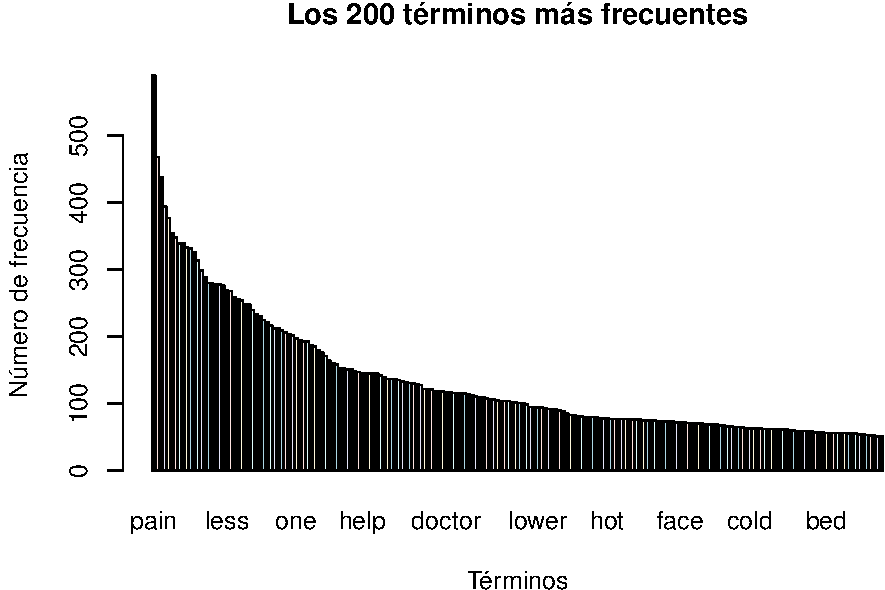
\includegraphics{practica_files/figure-latex/unnamed-chunk-22-1.pdf}

Una vez que tenemos los 100 términos con mayor frecuencia en nuestra
columna \emph{benefitsReview} y su frecuencia asociada, pasamos a matriz
dichos datos, con el fin de obtener solo las palabras y descartar su
frecuencia.

\begin{Shaded}
\begin{Highlighting}[]
\CommentTok{# Convertimos a matriz "terms_frecuency_benefits_corpus_100"}
\NormalTok{terms_frecuency_benefits_train_corpus_}\DecValTok{200}\NormalTok{ <-}\StringTok{ }\KeywordTok{as.matrix}\NormalTok{(terms_frecuency_benefits_train_corpus_}\DecValTok{200}\NormalTok{)}
\NormalTok{terms_frecuency_benefits_train_corpus_}\DecValTok{200}
\end{Highlighting}
\end{Shaded}

\begin{verbatim}
##               [,1]
## pain           590
## taking         468
## drug           438
## also           394
## day            377
## skin           355
## sleep          348
## treatment      339
## able           339
## medication     333
## time           332
## better         326
## effects        314
## take           299
## much           289
## feel           280
## get            279
## symptoms       278
## depression     278
## helped         276
## less           269
## side           268
## years          259
## reduced        256
## benefits       254
## days           249
## acne           248
## first          240
## felt           233
## without        231
## anxiety        225
## life           222
## within         217
## still          212
## like           212
## now            209
## effective      206
## took           204
## started        202
## one            197
## work           195
## back           193
## months         193
## night          187
## weeks          185
## blood          180
## well           176
## can            171
## stopped        164
## severe         160
## just           158
## used           152
## even           152
## normal         151
## two            151
## taken          148
## feeling        147
## help           146
## improved       145
## mood           145
## hours          145
## increased      145
## made           142
## pressure       139
## control        137
## good           137
## didnt          137
## went           135
## hair           133
## cleared        132
## energy         131
## week           130
## really         129
## use            128
## completely     122
## daily          122
## almost         121
## weight         119
## prescribed     118
## reduction      118
## doctor         117
## infection      117
## dose           116
## away           115
## decreased      115
## times          115
## due            114
## relief         113
## none           111
## long           110
## however        110
## year           108
## will           106
## since          106
## every          105
## effect         104
## dont           104
## little         104
## longer         102
## patient        102
## loss           101
## never          101
## worked          99
## noticed         95
## seemed          94
## lower           94
## benefit         94
## using           93
## experienced     92
## month           91
## headaches       91
## tried           90
## think           88
## gone            85
## got             83
## high            82
## period          81
## medicine        81
## overall         80
## pill            80
## ive             80
## getting         79
## great           78
## stop            78
## hot             78
## began           77
## many            77
## migraine        77
## mild            77
## improvement     77
## reduce          76
## decrease        76
## things          76
## levels          76
## dosage          75
## problems        75
## found           75
## going           75
## results         74
## need            74
## acid            73
## became          73
## focus           73
## experience      72
## face            72
## clear           72
## around          71
## condition       71
## panic           70
## function        70
## several         70
## helps           69
## level           69
## morning         69
## cholesterol     69
## heart           67
## quickly         67
## asleep          66
## significantly   66
## though          65
## make            65
## attacks         64
## know            63
## cold            63
## per             63
## problem         63
## see             63
## although        62
## increase        62
## eliminated      62
## three           61
## works           61
## eyes            61
## bad             61
## immediately     60
## headache        60
## usually         59
## difference      59
## caused          59
## worse           58
## flashes         58
## starting        57
## stomach         57
## ability         57
## bed             56
## reflux          56
## migraines       56
## drugs           56
## dry             56
## allowed         56
## another         55
## new             55
## gave            55
## body            54
## easy            54
## smoking         53
## last            52
## lowered         52
## enough          51
## etc             51
\end{verbatim}

\begin{Shaded}
\begin{Highlighting}[]
\CommentTok{# Me quedo solo con los términos}
\NormalTok{terms_benefits_train_corpus_}\DecValTok{200}\NormalTok{ <-}\StringTok{ }\KeywordTok{rownames}\NormalTok{(terms_frecuency_benefits_train_corpus_}\DecValTok{200}\NormalTok{)}
\NormalTok{terms_benefits_train_corpus_}\DecValTok{200}
\end{Highlighting}
\end{Shaded}

\begin{verbatim}
##   [1] "pain"          "taking"        "drug"          "also"         
##   [5] "day"           "skin"          "sleep"         "treatment"    
##   [9] "able"          "medication"    "time"          "better"       
##  [13] "effects"       "take"          "much"          "feel"         
##  [17] "get"           "symptoms"      "depression"    "helped"       
##  [21] "less"          "side"          "years"         "reduced"      
##  [25] "benefits"      "days"          "acne"          "first"        
##  [29] "felt"          "without"       "anxiety"       "life"         
##  [33] "within"        "still"         "like"          "now"          
##  [37] "effective"     "took"          "started"       "one"          
##  [41] "work"          "back"          "months"        "night"        
##  [45] "weeks"         "blood"         "well"          "can"          
##  [49] "stopped"       "severe"        "just"          "used"         
##  [53] "even"          "normal"        "two"           "taken"        
##  [57] "feeling"       "help"          "improved"      "mood"         
##  [61] "hours"         "increased"     "made"          "pressure"     
##  [65] "control"       "good"          "didnt"         "went"         
##  [69] "hair"          "cleared"       "energy"        "week"         
##  [73] "really"        "use"           "completely"    "daily"        
##  [77] "almost"        "weight"        "prescribed"    "reduction"    
##  [81] "doctor"        "infection"     "dose"          "away"         
##  [85] "decreased"     "times"         "due"           "relief"       
##  [89] "none"          "long"          "however"       "year"         
##  [93] "will"          "since"         "every"         "effect"       
##  [97] "dont"          "little"        "longer"        "patient"      
## [101] "loss"          "never"         "worked"        "noticed"      
## [105] "seemed"        "lower"         "benefit"       "using"        
## [109] "experienced"   "month"         "headaches"     "tried"        
## [113] "think"         "gone"          "got"           "high"         
## [117] "period"        "medicine"      "overall"       "pill"         
## [121] "ive"           "getting"       "great"         "stop"         
## [125] "hot"           "began"         "many"          "migraine"     
## [129] "mild"          "improvement"   "reduce"        "decrease"     
## [133] "things"        "levels"        "dosage"        "problems"     
## [137] "found"         "going"         "results"       "need"         
## [141] "acid"          "became"        "focus"         "experience"   
## [145] "face"          "clear"         "around"        "condition"    
## [149] "panic"         "function"      "several"       "helps"        
## [153] "level"         "morning"       "cholesterol"   "heart"        
## [157] "quickly"       "asleep"        "significantly" "though"       
## [161] "make"          "attacks"       "know"          "cold"         
## [165] "per"           "problem"       "see"           "although"     
## [169] "increase"      "eliminated"    "three"         "works"        
## [173] "eyes"          "bad"           "immediately"   "headache"     
## [177] "usually"       "difference"    "caused"        "worse"        
## [181] "flashes"       "starting"      "stomach"       "ability"      
## [185] "bed"           "reflux"        "migraines"     "drugs"        
## [189] "dry"           "allowed"       "another"       "new"          
## [193] "gave"          "body"          "easy"          "smoking"      
## [197] "last"          "lowered"       "enough"        "etc"
\end{verbatim}

Como ya sabemos las palabras a usar, es decir, los 100 términos que más
se repite, procedemos a la agrupación por sinónimos. En donde, mediante
la función \emph{distance(\ldots{})} de la libería \emph{rword2vec},
obtendremos todas palabras más similares de nuestro conjunto, en nuestro
caso nos vamos a quedar con las 2 primeras:

\begin{Shaded}
\begin{Highlighting}[]
\CommentTok{# http://mccormickml.com/2016/04/12/googles-pretrained-word2vec-model-in-python/}
\CommentTok{# https://github.com/mukul13/rword2vec}
\CommentTok{# http://www.rpubs.com/mukul13/rword2vec}

\KeywordTok{library}\NormalTok{(devtools)                   }\CommentTok{# hace falta esta librería para que funcione}
\KeywordTok{install_github}\NormalTok{(}\StringTok{"mukul13/rword2vec"}\NormalTok{) }\CommentTok{# nos instalamos la libreria desde Github}
\end{Highlighting}
\end{Shaded}

\begin{verbatim}
## Skipping install of 'rword2vec' from a github remote, the SHA1 (9942d70f) has not changed since last install.
##   Use `force = TRUE` to force installation
\end{verbatim}

\begin{Shaded}
\begin{Highlighting}[]
\KeywordTok{library}\NormalTok{(rword2vec)}

\CommentTok{# Escribo en un fichero la columna "benefitsReview"}
\KeywordTok{write.table}\NormalTok{(datos_train}\OperatorTok{$}\NormalTok{benefitsReview, }\StringTok{"benefitsReview.txt"}\NormalTok{, }\DataTypeTok{sep =} \StringTok{"}\CharTok{\textbackslash{}t}\StringTok{"}\NormalTok{, }\DataTypeTok{quote =}\NormalTok{ F, }\DataTypeTok{row.names =}\NormalTok{ F)}

\CommentTok{# Entreno los datos del texto para obtener los vectores de palabras}
\NormalTok{model_benefits_train =}\StringTok{ }\KeywordTok{word2vec}\NormalTok{(}\DataTypeTok{train_file =} \StringTok{"benefitsReview.txt"}\NormalTok{, }\DataTypeTok{output_file =} \StringTok{"benefitsReview.bin"}\NormalTok{, }\DataTypeTok{binary=}\DecValTok{1}\NormalTok{)}
\end{Highlighting}
\end{Shaded}

\begin{verbatim}
## Starting training using file benefitsReview.txt
## 100K
Vocab size: 2314
## Words in train file: 100690
\end{verbatim}

\begin{Shaded}
\begin{Highlighting}[]
\NormalTok{dist_terms_benefits_train_corpus_}\DecValTok{200}\NormalTok{ =}\StringTok{ }\KeywordTok{c}\NormalTok{()}
\CommentTok{# Obtengo la distancia de las 100 palabras con mayor frecuencia}
\ControlFlowTok{for}\NormalTok{ (i }\ControlFlowTok{in} \DecValTok{1}\OperatorTok{:}\KeywordTok{length}\NormalTok{(terms_benefits_train_corpus_}\DecValTok{200}\NormalTok{))\{ }\CommentTok{# calculamos la distancia de la palabra a sus sinónimos}
\NormalTok{  dist_terms_benefits_train_corpus_}\DecValTok{200}\NormalTok{[i] =}\StringTok{ }\KeywordTok{distance}\NormalTok{(}\DataTypeTok{file_name =} \StringTok{"benefitsReview.bin"}\NormalTok{, }\DataTypeTok{search_word =}\NormalTok{ terms_benefits_train_corpus_}\DecValTok{200}\NormalTok{[i], }\DataTypeTok{num =} \DecValTok{2}\NormalTok{)}
\NormalTok{\}}
\end{Highlighting}
\end{Shaded}

\begin{verbatim}
## Entered word or sentence: pain
## 
## Word: pain  Position in vocabulary: 29
\end{verbatim}

\begin{verbatim}
## Warning in dist_terms_benefits_train_corpus_200[i] <- distance(file_name
## = "benefitsReview.bin", : número de items para para sustituir no es un
## múltiplo de la longitud del reemplazo
\end{verbatim}

\begin{verbatim}
## Entered word or sentence: taking
## 
## Word: taking  Position in vocabulary: 28
\end{verbatim}

\begin{verbatim}
## Warning in dist_terms_benefits_train_corpus_200[i] <- distance(file_name
## = "benefitsReview.bin", : número de items para para sustituir no es un
## múltiplo de la longitud del reemplazo
\end{verbatim}

\begin{verbatim}
## Entered word or sentence: drug
## 
## Word: drug  Position in vocabulary: 38
\end{verbatim}

\begin{verbatim}
## Warning in dist_terms_benefits_train_corpus_200[i] <- distance(file_name
## = "benefitsReview.bin", : número de items para para sustituir no es un
## múltiplo de la longitud del reemplazo
\end{verbatim}

\begin{verbatim}
## Entered word or sentence: also
## 
## Word: also  Position in vocabulary: 41
\end{verbatim}

\begin{verbatim}
## Warning in dist_terms_benefits_train_corpus_200[i] <- distance(file_name
## = "benefitsReview.bin", : número de items para para sustituir no es un
## múltiplo de la longitud del reemplazo
\end{verbatim}

\begin{verbatim}
## Entered word or sentence: day
## 
## Word: day  Position in vocabulary: 74
\end{verbatim}

\begin{verbatim}
## Warning in dist_terms_benefits_train_corpus_200[i] <- distance(file_name
## = "benefitsReview.bin", : número de items para para sustituir no es un
## múltiplo de la longitud del reemplazo
\end{verbatim}

\begin{verbatim}
## Entered word or sentence: skin
## 
## Word: skin  Position in vocabulary: 50
\end{verbatim}

\begin{verbatim}
## Warning in dist_terms_benefits_train_corpus_200[i] <- distance(file_name
## = "benefitsReview.bin", : número de items para para sustituir no es un
## múltiplo de la longitud del reemplazo
\end{verbatim}

\begin{verbatim}
## Entered word or sentence: sleep
## 
## Word: sleep  Position in vocabulary: 60
\end{verbatim}

\begin{verbatim}
## Warning in dist_terms_benefits_train_corpus_200[i] <- distance(file_name
## = "benefitsReview.bin", : número de items para para sustituir no es un
## múltiplo de la longitud del reemplazo
\end{verbatim}

\begin{verbatim}
## Entered word or sentence: treatment
## 
## Word: treatment  Position in vocabulary: 61
\end{verbatim}

\begin{verbatim}
## Warning in dist_terms_benefits_train_corpus_200[i] <- distance(file_name
## = "benefitsReview.bin", : número de items para para sustituir no es un
## múltiplo de la longitud del reemplazo
\end{verbatim}

\begin{verbatim}
## Entered word or sentence: able
## 
## Word: able  Position in vocabulary: 42
\end{verbatim}

\begin{verbatim}
## Warning in dist_terms_benefits_train_corpus_200[i] <- distance(file_name
## = "benefitsReview.bin", : número de items para para sustituir no es un
## múltiplo de la longitud del reemplazo
\end{verbatim}

\begin{verbatim}
## Entered word or sentence: medication
## 
## Word: medication  Position in vocabulary: 66
\end{verbatim}

\begin{verbatim}
## Warning in dist_terms_benefits_train_corpus_200[i] <- distance(file_name
## = "benefitsReview.bin", : número de items para para sustituir no es un
## múltiplo de la longitud del reemplazo
\end{verbatim}

\begin{verbatim}
## Entered word or sentence: time
## 
## Word: time  Position in vocabulary: 69
\end{verbatim}

\begin{verbatim}
## Warning in dist_terms_benefits_train_corpus_200[i] <- distance(file_name
## = "benefitsReview.bin", : número de items para para sustituir no es un
## múltiplo de la longitud del reemplazo
\end{verbatim}

\begin{verbatim}
## Entered word or sentence: better
## 
## Word: better  Position in vocabulary: 70
\end{verbatim}

\begin{verbatim}
## Warning in dist_terms_benefits_train_corpus_200[i] <- distance(file_name
## = "benefitsReview.bin", : número de items para para sustituir no es un
## múltiplo de la longitud del reemplazo
\end{verbatim}

\begin{verbatim}
## Entered word or sentence: effects
## 
## Word: effects  Position in vocabulary: 73
\end{verbatim}

\begin{verbatim}
## Warning in dist_terms_benefits_train_corpus_200[i] <- distance(file_name
## = "benefitsReview.bin", : número de items para para sustituir no es un
## múltiplo de la longitud del reemplazo
\end{verbatim}

\begin{verbatim}
## Entered word or sentence: take
## 
## Word: take  Position in vocabulary: 48
\end{verbatim}

\begin{verbatim}
## Warning in dist_terms_benefits_train_corpus_200[i] <- distance(file_name
## = "benefitsReview.bin", : número de items para para sustituir no es un
## múltiplo de la longitud del reemplazo
\end{verbatim}

\begin{verbatim}
## Entered word or sentence: much
## 
## Word: much  Position in vocabulary: 59
\end{verbatim}

\begin{verbatim}
## Warning in dist_terms_benefits_train_corpus_200[i] <- distance(file_name
## = "benefitsReview.bin", : número de items para para sustituir no es un
## múltiplo de la longitud del reemplazo
\end{verbatim}

\begin{verbatim}
## Entered word or sentence: feel
## 
## Word: feel  Position in vocabulary: 52
\end{verbatim}

\begin{verbatim}
## Warning in dist_terms_benefits_train_corpus_200[i] <- distance(file_name
## = "benefitsReview.bin", : número de items para para sustituir no es un
## múltiplo de la longitud del reemplazo
\end{verbatim}

\begin{verbatim}
## Entered word or sentence: get
## 
## Word: get  Position in vocabulary: 51
\end{verbatim}

\begin{verbatim}
## Warning in dist_terms_benefits_train_corpus_200[i] <- distance(file_name
## = "benefitsReview.bin", : número de items para para sustituir no es un
## múltiplo de la longitud del reemplazo
\end{verbatim}

\begin{verbatim}
## Entered word or sentence: symptoms
## 
## Word: symptoms  Position in vocabulary: 72
\end{verbatim}

\begin{verbatim}
## Warning in dist_terms_benefits_train_corpus_200[i] <- distance(file_name
## = "benefitsReview.bin", : número de items para para sustituir no es un
## múltiplo de la longitud del reemplazo
\end{verbatim}

\begin{verbatim}
## Entered word or sentence: depression
## 
## Word: depression  Position in vocabulary: 96
\end{verbatim}

\begin{verbatim}
## Warning in dist_terms_benefits_train_corpus_200[i] <- distance(file_name
## = "benefitsReview.bin", : número de items para para sustituir no es un
## múltiplo de la longitud del reemplazo
\end{verbatim}

\begin{verbatim}
## Entered word or sentence: helped
## 
## Word: helped  Position in vocabulary: 62
\end{verbatim}

\begin{verbatim}
## Warning in dist_terms_benefits_train_corpus_200[i] <- distance(file_name
## = "benefitsReview.bin", : número de items para para sustituir no es un
## múltiplo de la longitud del reemplazo
\end{verbatim}

\begin{verbatim}
## Entered word or sentence: less
## 
## Word: less  Position in vocabulary: 64
\end{verbatim}

\begin{verbatim}
## Warning in dist_terms_benefits_train_corpus_200[i] <- distance(file_name
## = "benefitsReview.bin", : número de items para para sustituir no es un
## múltiplo de la longitud del reemplazo
\end{verbatim}

\begin{verbatim}
## Entered word or sentence: side
## 
## Word: side  Position in vocabulary: 54
\end{verbatim}

\begin{verbatim}
## Warning in dist_terms_benefits_train_corpus_200[i] <- distance(file_name
## = "benefitsReview.bin", : número de items para para sustituir no es un
## múltiplo de la longitud del reemplazo
\end{verbatim}

\begin{verbatim}
## Entered word or sentence: years
## 
## Word: years  Position in vocabulary: 98
\end{verbatim}

\begin{verbatim}
## Warning in dist_terms_benefits_train_corpus_200[i] <- distance(file_name
## = "benefitsReview.bin", : número de items para para sustituir no es un
## múltiplo de la longitud del reemplazo
\end{verbatim}

\begin{verbatim}
## Entered word or sentence: reduced
## 
## Word: reduced  Position in vocabulary: 78
\end{verbatim}

\begin{verbatim}
## Warning in dist_terms_benefits_train_corpus_200[i] <- distance(file_name
## = "benefitsReview.bin", : número de items para para sustituir no es un
## múltiplo de la longitud del reemplazo
\end{verbatim}

\begin{verbatim}
## Entered word or sentence: benefits
## 
## Word: benefits  Position in vocabulary: 85
\end{verbatim}

\begin{verbatim}
## Warning in dist_terms_benefits_train_corpus_200[i] <- distance(file_name
## = "benefitsReview.bin", : número de items para para sustituir no es un
## múltiplo de la longitud del reemplazo
\end{verbatim}

\begin{verbatim}
## Entered word or sentence: days
## 
## Word: days  Position in vocabulary: 99
\end{verbatim}

\begin{verbatim}
## Warning in dist_terms_benefits_train_corpus_200[i] <- distance(file_name
## = "benefitsReview.bin", : número de items para para sustituir no es un
## múltiplo de la longitud del reemplazo
\end{verbatim}

\begin{verbatim}
## Entered word or sentence: acne
## 
## Word: acne  Position in vocabulary: 93
\end{verbatim}

\begin{verbatim}
## Warning in dist_terms_benefits_train_corpus_200[i] <- distance(file_name
## = "benefitsReview.bin", : número de items para para sustituir no es un
## múltiplo de la longitud del reemplazo
\end{verbatim}

\begin{verbatim}
## Entered word or sentence: first
## 
## Word: first  Position in vocabulary: 67
\end{verbatim}

\begin{verbatim}
## Warning in dist_terms_benefits_train_corpus_200[i] <- distance(file_name
## = "benefitsReview.bin", : número de items para para sustituir no es un
## múltiplo de la longitud del reemplazo
\end{verbatim}

\begin{verbatim}
## Entered word or sentence: felt
## 
## Word: felt  Position in vocabulary: 65
\end{verbatim}

\begin{verbatim}
## Warning in dist_terms_benefits_train_corpus_200[i] <- distance(file_name
## = "benefitsReview.bin", : número de items para para sustituir no es un
## múltiplo de la longitud del reemplazo
\end{verbatim}

\begin{verbatim}
## Entered word or sentence: without
## 
## Word: without  Position in vocabulary: 71
\end{verbatim}

\begin{verbatim}
## Warning in dist_terms_benefits_train_corpus_200[i] <- distance(file_name
## = "benefitsReview.bin", : número de items para para sustituir no es un
## múltiplo de la longitud del reemplazo
\end{verbatim}

\begin{verbatim}
## Entered word or sentence: anxiety
## 
## Word: anxiety  Position in vocabulary: 110
\end{verbatim}

\begin{verbatim}
## Warning in dist_terms_benefits_train_corpus_200[i] <- distance(file_name
## = "benefitsReview.bin", : número de items para para sustituir no es un
## múltiplo de la longitud del reemplazo
\end{verbatim}

\begin{verbatim}
## Entered word or sentence: life
## 
## Word: life  Position in vocabulary: 123
\end{verbatim}

\begin{verbatim}
## Warning in dist_terms_benefits_train_corpus_200[i] <- distance(file_name
## = "benefitsReview.bin", : número de items para para sustituir no es un
## múltiplo de la longitud del reemplazo
\end{verbatim}

\begin{verbatim}
## Entered word or sentence: within
## 
## Word: within  Position in vocabulary: 83
\end{verbatim}

\begin{verbatim}
## Warning in dist_terms_benefits_train_corpus_200[i] <- distance(file_name
## = "benefitsReview.bin", : número de items para para sustituir no es un
## múltiplo de la longitud del reemplazo
\end{verbatim}

\begin{verbatim}
## Entered word or sentence: still
## 
## Word: still  Position in vocabulary: 75
\end{verbatim}

\begin{verbatim}
## Warning in dist_terms_benefits_train_corpus_200[i] <- distance(file_name
## = "benefitsReview.bin", : número de items para para sustituir no es un
## múltiplo de la longitud del reemplazo
\end{verbatim}

\begin{verbatim}
## Entered word or sentence: like
## 
## Word: like  Position in vocabulary: 76
\end{verbatim}

\begin{verbatim}
## Warning in dist_terms_benefits_train_corpus_200[i] <- distance(file_name
## = "benefitsReview.bin", : número de items para para sustituir no es un
## múltiplo de la longitud del reemplazo
\end{verbatim}

\begin{verbatim}
## Entered word or sentence: now
## 
## Word: now  Position in vocabulary: 112
\end{verbatim}

\begin{verbatim}
## Warning in dist_terms_benefits_train_corpus_200[i] <- distance(file_name
## = "benefitsReview.bin", : número de items para para sustituir no es un
## múltiplo de la longitud del reemplazo
\end{verbatim}

\begin{verbatim}
## Entered word or sentence: effective
## 
## Word: effective  Position in vocabulary: 97
\end{verbatim}

\begin{verbatim}
## Warning in dist_terms_benefits_train_corpus_200[i] <- distance(file_name
## = "benefitsReview.bin", : número de items para para sustituir no es un
## múltiplo de la longitud del reemplazo
\end{verbatim}

\begin{verbatim}
## Entered word or sentence: took
## 
## Word: took  Position in vocabulary: 80
\end{verbatim}

\begin{verbatim}
## Warning in dist_terms_benefits_train_corpus_200[i] <- distance(file_name
## = "benefitsReview.bin", : número de items para para sustituir no es un
## múltiplo de la longitud del reemplazo
\end{verbatim}

\begin{verbatim}
## Entered word or sentence: started
## 
## Word: started  Position in vocabulary: 84
\end{verbatim}

\begin{verbatim}
## Warning in dist_terms_benefits_train_corpus_200[i] <- distance(file_name
## = "benefitsReview.bin", : número de items para para sustituir no es un
## múltiplo de la longitud del reemplazo
\end{verbatim}

\begin{verbatim}
## Entered word or sentence: one
## 
## Word: one  Position in vocabulary: 94
\end{verbatim}

\begin{verbatim}
## Warning in dist_terms_benefits_train_corpus_200[i] <- distance(file_name
## = "benefitsReview.bin", : número de items para para sustituir no es un
## múltiplo de la longitud del reemplazo
\end{verbatim}

\begin{verbatim}
## Entered word or sentence: work
## 
## Word: work  Position in vocabulary: 111
\end{verbatim}

\begin{verbatim}
## Warning in dist_terms_benefits_train_corpus_200[i] <- distance(file_name
## = "benefitsReview.bin", : número de items para para sustituir no es un
## múltiplo de la longitud del reemplazo
\end{verbatim}

\begin{verbatim}
## Entered word or sentence: back
## 
## Word: back  Position in vocabulary: 102
\end{verbatim}

\begin{verbatim}
## Warning in dist_terms_benefits_train_corpus_200[i] <- distance(file_name
## = "benefitsReview.bin", : número de items para para sustituir no es un
## múltiplo de la longitud del reemplazo
\end{verbatim}

\begin{verbatim}
## Entered word or sentence: months
## 
## Word: months  Position in vocabulary: 114
\end{verbatim}

\begin{verbatim}
## Warning in dist_terms_benefits_train_corpus_200[i] <- distance(file_name
## = "benefitsReview.bin", : número de items para para sustituir no es un
## múltiplo de la longitud del reemplazo
\end{verbatim}

\begin{verbatim}
## Entered word or sentence: night
## 
## Word: night  Position in vocabulary: 135
\end{verbatim}

\begin{verbatim}
## Warning in dist_terms_benefits_train_corpus_200[i] <- distance(file_name
## = "benefitsReview.bin", : número de items para para sustituir no es un
## múltiplo de la longitud del reemplazo
\end{verbatim}

\begin{verbatim}
## Entered word or sentence: weeks
## 
## Word: weeks  Position in vocabulary: 130
\end{verbatim}

\begin{verbatim}
## Warning in dist_terms_benefits_train_corpus_200[i] <- distance(file_name
## = "benefitsReview.bin", : número de items para para sustituir no es un
## múltiplo de la longitud del reemplazo
\end{verbatim}

\begin{verbatim}
## Entered word or sentence: blood
## 
## Word: blood  Position in vocabulary: 91
\end{verbatim}

\begin{verbatim}
## Warning in dist_terms_benefits_train_corpus_200[i] <- distance(file_name
## = "benefitsReview.bin", : número de items para para sustituir no es un
## múltiplo de la longitud del reemplazo
\end{verbatim}

\begin{verbatim}
## Entered word or sentence: well
## 
## Word: well  Position in vocabulary: 139
\end{verbatim}

\begin{verbatim}
## Warning in dist_terms_benefits_train_corpus_200[i] <- distance(file_name
## = "benefitsReview.bin", : número de items para para sustituir no es un
## múltiplo de la longitud del reemplazo
\end{verbatim}

\begin{verbatim}
## Entered word or sentence: can
## 
## Word: can  Position in vocabulary: 92
\end{verbatim}

\begin{verbatim}
## Warning in dist_terms_benefits_train_corpus_200[i] <- distance(file_name
## = "benefitsReview.bin", : número de items para para sustituir no es un
## múltiplo de la longitud del reemplazo
\end{verbatim}

\begin{verbatim}
## Entered word or sentence: stopped
## 
## Word: stopped  Position in vocabulary: 119
\end{verbatim}

\begin{verbatim}
## Warning in dist_terms_benefits_train_corpus_200[i] <- distance(file_name
## = "benefitsReview.bin", : número de items para para sustituir no es un
## múltiplo de la longitud del reemplazo
\end{verbatim}

\begin{verbatim}
## Entered word or sentence: severe
## 
## Word: severe  Position in vocabulary: 107
\end{verbatim}

\begin{verbatim}
## Warning in dist_terms_benefits_train_corpus_200[i] <- distance(file_name
## = "benefitsReview.bin", : número de items para para sustituir no es un
## múltiplo de la longitud del reemplazo
\end{verbatim}

\begin{verbatim}
## Entered word or sentence: just
## 
## Word: just  Position in vocabulary: 103
\end{verbatim}

\begin{verbatim}
## Warning in dist_terms_benefits_train_corpus_200[i] <- distance(file_name
## = "benefitsReview.bin", : número de items para para sustituir no es un
## múltiplo de la longitud del reemplazo
\end{verbatim}

\begin{verbatim}
## Entered word or sentence: used
## 
## Word: used  Position in vocabulary: 106
\end{verbatim}

\begin{verbatim}
## Warning in dist_terms_benefits_train_corpus_200[i] <- distance(file_name
## = "benefitsReview.bin", : número de items para para sustituir no es un
## múltiplo de la longitud del reemplazo
\end{verbatim}

\begin{verbatim}
## Entered word or sentence: even
## 
## Word: even  Position in vocabulary: 115
\end{verbatim}

\begin{verbatim}
## Warning in dist_terms_benefits_train_corpus_200[i] <- distance(file_name
## = "benefitsReview.bin", : número de items para para sustituir no es un
## múltiplo de la longitud del reemplazo
\end{verbatim}

\begin{verbatim}
## Entered word or sentence: normal
## 
## Word: normal  Position in vocabulary: 141
\end{verbatim}

\begin{verbatim}
## Warning in dist_terms_benefits_train_corpus_200[i] <- distance(file_name
## = "benefitsReview.bin", : número de items para para sustituir no es un
## múltiplo de la longitud del reemplazo
\end{verbatim}

\begin{verbatim}
## Entered word or sentence: two
## 
## Word: two  Position in vocabulary: 109
\end{verbatim}

\begin{verbatim}
## Warning in dist_terms_benefits_train_corpus_200[i] <- distance(file_name
## = "benefitsReview.bin", : número de items para para sustituir no es un
## múltiplo de la longitud del reemplazo
\end{verbatim}

\begin{verbatim}
## Entered word or sentence: taken
## 
## Word: taken  Position in vocabulary: 117
\end{verbatim}

\begin{verbatim}
## Warning in dist_terms_benefits_train_corpus_200[i] <- distance(file_name
## = "benefitsReview.bin", : número de items para para sustituir no es un
## múltiplo de la longitud del reemplazo
\end{verbatim}

\begin{verbatim}
## Entered word or sentence: feeling
## 
## Word: feeling  Position in vocabulary: 113
\end{verbatim}

\begin{verbatim}
## Warning in dist_terms_benefits_train_corpus_200[i] <- distance(file_name
## = "benefitsReview.bin", : número de items para para sustituir no es un
## múltiplo de la longitud del reemplazo
\end{verbatim}

\begin{verbatim}
## Entered word or sentence: help
## 
## Word: help  Position in vocabulary: 120
\end{verbatim}

\begin{verbatim}
## Warning in dist_terms_benefits_train_corpus_200[i] <- distance(file_name
## = "benefitsReview.bin", : número de items para para sustituir no es un
## múltiplo de la longitud del reemplazo
\end{verbatim}

\begin{verbatim}
## Entered word or sentence: improved
## 
## Word: improved  Position in vocabulary: 149
\end{verbatim}

\begin{verbatim}
## Warning in dist_terms_benefits_train_corpus_200[i] <- distance(file_name
## = "benefitsReview.bin", : número de items para para sustituir no es un
## múltiplo de la longitud del reemplazo
\end{verbatim}

\begin{verbatim}
## Entered word or sentence: mood
## 
## Word: mood  Position in vocabulary: 161
\end{verbatim}

\begin{verbatim}
## Warning in dist_terms_benefits_train_corpus_200[i] <- distance(file_name
## = "benefitsReview.bin", : número de items para para sustituir no es un
## múltiplo de la longitud del reemplazo
\end{verbatim}

\begin{verbatim}
## Entered word or sentence: hours
## 
## Word: hours  Position in vocabulary: 166
\end{verbatim}

\begin{verbatim}
## Warning in dist_terms_benefits_train_corpus_200[i] <- distance(file_name
## = "benefitsReview.bin", : número de items para para sustituir no es un
## múltiplo de la longitud del reemplazo
\end{verbatim}

\begin{verbatim}
## Entered word or sentence: increased
## 
## Word: increased  Position in vocabulary: 138
\end{verbatim}

\begin{verbatim}
## Warning in dist_terms_benefits_train_corpus_200[i] <- distance(file_name
## = "benefitsReview.bin", : número de items para para sustituir no es un
## múltiplo de la longitud del reemplazo
\end{verbatim}

\begin{verbatim}
## Entered word or sentence: made
## 
## Word: made  Position in vocabulary: 121
\end{verbatim}

\begin{verbatim}
## Warning in dist_terms_benefits_train_corpus_200[i] <- distance(file_name
## = "benefitsReview.bin", : número de items para para sustituir no es un
## múltiplo de la longitud del reemplazo
\end{verbatim}

\begin{verbatim}
## Entered word or sentence: pressure
## 
## Word: pressure  Position in vocabulary: 131
\end{verbatim}

\begin{verbatim}
## Warning in dist_terms_benefits_train_corpus_200[i] <- distance(file_name
## = "benefitsReview.bin", : número de items para para sustituir no es un
## múltiplo de la longitud del reemplazo
\end{verbatim}

\begin{verbatim}
## Entered word or sentence: control
## 
## Word: control  Position in vocabulary: 154
\end{verbatim}

\begin{verbatim}
## Warning in dist_terms_benefits_train_corpus_200[i] <- distance(file_name
## = "benefitsReview.bin", : número de items para para sustituir no es un
## múltiplo de la longitud del reemplazo
\end{verbatim}

\begin{verbatim}
## Entered word or sentence: good
## 
## Word: good  Position in vocabulary: 140
\end{verbatim}

\begin{verbatim}
## Warning in dist_terms_benefits_train_corpus_200[i] <- distance(file_name
## = "benefitsReview.bin", : número de items para para sustituir no es un
## múltiplo de la longitud del reemplazo
\end{verbatim}

\begin{verbatim}
## Entered word or sentence: didnt
## 
## Word: didnt  Position in vocabulary: 1007
\end{verbatim}

\begin{verbatim}
## Warning in dist_terms_benefits_train_corpus_200[i] <- distance(file_name
## = "benefitsReview.bin", : número de items para para sustituir no es un
## múltiplo de la longitud del reemplazo
\end{verbatim}

\begin{verbatim}
## Entered word or sentence: went
## 
## Word: went  Position in vocabulary: 122
\end{verbatim}

\begin{verbatim}
## Warning in dist_terms_benefits_train_corpus_200[i] <- distance(file_name
## = "benefitsReview.bin", : número de items para para sustituir no es un
## múltiplo de la longitud del reemplazo
\end{verbatim}

\begin{verbatim}
## Entered word or sentence: hair
## 
## Word: hair  Position in vocabulary: 137
\end{verbatim}

\begin{verbatim}
## Warning in dist_terms_benefits_train_corpus_200[i] <- distance(file_name
## = "benefitsReview.bin", : número de items para para sustituir no es un
## múltiplo de la longitud del reemplazo
\end{verbatim}

\begin{verbatim}
## Entered word or sentence: cleared
## 
## Word: cleared  Position in vocabulary: 136
\end{verbatim}

\begin{verbatim}
## Warning in dist_terms_benefits_train_corpus_200[i] <- distance(file_name
## = "benefitsReview.bin", : número de items para para sustituir no es un
## múltiplo de la longitud del reemplazo
\end{verbatim}

\begin{verbatim}
## Entered word or sentence: energy
## 
## Word: energy  Position in vocabulary: 185
\end{verbatim}

\begin{verbatim}
## Warning in dist_terms_benefits_train_corpus_200[i] <- distance(file_name
## = "benefitsReview.bin", : número de items para para sustituir no es un
## múltiplo de la longitud del reemplazo
\end{verbatim}

\begin{verbatim}
## Entered word or sentence: week
## 
## Word: week  Position in vocabulary: 187
\end{verbatim}

\begin{verbatim}
## Warning in dist_terms_benefits_train_corpus_200[i] <- distance(file_name
## = "benefitsReview.bin", : número de items para para sustituir no es un
## múltiplo de la longitud del reemplazo
\end{verbatim}

\begin{verbatim}
## Entered word or sentence: really
## 
## Word: really  Position in vocabulary: 127
\end{verbatim}

\begin{verbatim}
## Warning in dist_terms_benefits_train_corpus_200[i] <- distance(file_name
## = "benefitsReview.bin", : número de items para para sustituir no es un
## múltiplo de la longitud del reemplazo
\end{verbatim}

\begin{verbatim}
## Entered word or sentence: use
## 
## Word: use  Position in vocabulary: 150
\end{verbatim}

\begin{verbatim}
## Warning in dist_terms_benefits_train_corpus_200[i] <- distance(file_name
## = "benefitsReview.bin", : número de items para para sustituir no es un
## múltiplo de la longitud del reemplazo
\end{verbatim}

\begin{verbatim}
## Entered word or sentence: completely
## 
## Word: completely  Position in vocabulary: 168
\end{verbatim}

\begin{verbatim}
## Warning in dist_terms_benefits_train_corpus_200[i] <- distance(file_name
## = "benefitsReview.bin", : número de items para para sustituir no es un
## múltiplo de la longitud del reemplazo
\end{verbatim}

\begin{verbatim}
## Entered word or sentence: daily
## 
## Word: daily  Position in vocabulary: 156
\end{verbatim}

\begin{verbatim}
## Warning in dist_terms_benefits_train_corpus_200[i] <- distance(file_name
## = "benefitsReview.bin", : número de items para para sustituir no es un
## múltiplo de la longitud del reemplazo
\end{verbatim}

\begin{verbatim}
## Entered word or sentence: almost
## 
## Word: almost  Position in vocabulary: 134
\end{verbatim}

\begin{verbatim}
## Warning in dist_terms_benefits_train_corpus_200[i] <- distance(file_name
## = "benefitsReview.bin", : número de items para para sustituir no es un
## múltiplo de la longitud del reemplazo
\end{verbatim}

\begin{verbatim}
## Entered word or sentence: weight
## 
## Word: weight  Position in vocabulary: 153
\end{verbatim}

\begin{verbatim}
## Warning in dist_terms_benefits_train_corpus_200[i] <- distance(file_name
## = "benefitsReview.bin", : número de items para para sustituir no es un
## múltiplo de la longitud del reemplazo
\end{verbatim}

\begin{verbatim}
## Entered word or sentence: prescribed
## 
## Word: prescribed  Position in vocabulary: 148
\end{verbatim}

\begin{verbatim}
## Warning in dist_terms_benefits_train_corpus_200[i] <- distance(file_name
## = "benefitsReview.bin", : número de items para para sustituir no es un
## múltiplo de la longitud del reemplazo
\end{verbatim}

\begin{verbatim}
## Entered word or sentence: reduction
## 
## Word: reduction  Position in vocabulary: 155
\end{verbatim}

\begin{verbatim}
## Warning in dist_terms_benefits_train_corpus_200[i] <- distance(file_name
## = "benefitsReview.bin", : número de items para para sustituir no es un
## múltiplo de la longitud del reemplazo
\end{verbatim}

\begin{verbatim}
## Entered word or sentence: doctor
## 
## Word: doctor  Position in vocabulary: 152
\end{verbatim}

\begin{verbatim}
## Warning in dist_terms_benefits_train_corpus_200[i] <- distance(file_name
## = "benefitsReview.bin", : número de items para para sustituir no es un
## múltiplo de la longitud del reemplazo
\end{verbatim}

\begin{verbatim}
## Entered word or sentence: infection
## 
## Word: infection  Position in vocabulary: 180
\end{verbatim}

\begin{verbatim}
## Warning in dist_terms_benefits_train_corpus_200[i] <- distance(file_name
## = "benefitsReview.bin", : número de items para para sustituir no es un
## múltiplo de la longitud del reemplazo
\end{verbatim}

\begin{verbatim}
## Entered word or sentence: dose
## 
## Word: dose  Position in vocabulary: 167
\end{verbatim}

\begin{verbatim}
## Warning in dist_terms_benefits_train_corpus_200[i] <- distance(file_name
## = "benefitsReview.bin", : número de items para para sustituir no es un
## múltiplo de la longitud del reemplazo
\end{verbatim}

\begin{verbatim}
## Entered word or sentence: away
## 
## Word: away  Position in vocabulary: 208
\end{verbatim}

\begin{verbatim}
## Warning in dist_terms_benefits_train_corpus_200[i] <- distance(file_name
## = "benefitsReview.bin", : número de items para para sustituir no es un
## múltiplo de la longitud del reemplazo
\end{verbatim}

\begin{verbatim}
## Entered word or sentence: decreased
## 
## Word: decreased  Position in vocabulary: 188
\end{verbatim}

\begin{verbatim}
## Warning in dist_terms_benefits_train_corpus_200[i] <- distance(file_name
## = "benefitsReview.bin", : número de items para para sustituir no es un
## múltiplo de la longitud del reemplazo
\end{verbatim}

\begin{verbatim}
## Entered word or sentence: times
## 
## Word: times  Position in vocabulary: 163
\end{verbatim}

\begin{verbatim}
## Warning in dist_terms_benefits_train_corpus_200[i] <- distance(file_name
## = "benefitsReview.bin", : número de items para para sustituir no es un
## múltiplo de la longitud del reemplazo
\end{verbatim}

\begin{verbatim}
## Entered word or sentence: due
## 
## Word: due  Position in vocabulary: 145
\end{verbatim}

\begin{verbatim}
## Warning in dist_terms_benefits_train_corpus_200[i] <- distance(file_name
## = "benefitsReview.bin", : número de items para para sustituir no es un
## múltiplo de la longitud del reemplazo
\end{verbatim}

\begin{verbatim}
## Entered word or sentence: relief
## 
## Word: relief  Position in vocabulary: 178
\end{verbatim}

\begin{verbatim}
## Warning in dist_terms_benefits_train_corpus_200[i] <- distance(file_name
## = "benefitsReview.bin", : número de items para para sustituir no es un
## múltiplo de la longitud del reemplazo
\end{verbatim}

\begin{verbatim}
## Entered word or sentence: none
## 
## Word: none  Position in vocabulary: 345
\end{verbatim}

\begin{verbatim}
## Warning in dist_terms_benefits_train_corpus_200[i] <- distance(file_name
## = "benefitsReview.bin", : número de items para para sustituir no es un
## múltiplo de la longitud del reemplazo
\end{verbatim}

\begin{verbatim}
## Entered word or sentence: long
## 
## Word: long  Position in vocabulary: 162
\end{verbatim}

\begin{verbatim}
## Warning in dist_terms_benefits_train_corpus_200[i] <- distance(file_name
## = "benefitsReview.bin", : número de items para para sustituir no es un
## múltiplo de la longitud del reemplazo
\end{verbatim}

\begin{verbatim}
## Entered word or sentence: however
## 
## Word: however  Position in vocabulary: 451
\end{verbatim}

\begin{verbatim}
## Warning in dist_terms_benefits_train_corpus_200[i] <- distance(file_name
## = "benefitsReview.bin", : número de items para para sustituir no es un
## múltiplo de la longitud del reemplazo
\end{verbatim}

\begin{verbatim}
## Entered word or sentence: year
## 
## Word: year  Position in vocabulary: 233
\end{verbatim}

\begin{verbatim}
## Warning in dist_terms_benefits_train_corpus_200[i] <- distance(file_name
## = "benefitsReview.bin", : número de items para para sustituir no es un
## múltiplo de la longitud del reemplazo
\end{verbatim}

\begin{verbatim}
## Entered word or sentence: will
## 
## Word: will  Position in vocabulary: 147
\end{verbatim}

\begin{verbatim}
## Warning in dist_terms_benefits_train_corpus_200[i] <- distance(file_name
## = "benefitsReview.bin", : número de items para para sustituir no es un
## múltiplo de la longitud del reemplazo
\end{verbatim}

\begin{verbatim}
## Entered word or sentence: since
## 
## Word: since  Position in vocabulary: 199
\end{verbatim}

\begin{verbatim}
## Warning in dist_terms_benefits_train_corpus_200[i] <- distance(file_name
## = "benefitsReview.bin", : número de items para para sustituir no es un
## múltiplo de la longitud del reemplazo
\end{verbatim}

\begin{verbatim}
## Entered word or sentence: every
## 
## Word: every  Position in vocabulary: 157
\end{verbatim}

\begin{verbatim}
## Warning in dist_terms_benefits_train_corpus_200[i] <- distance(file_name
## = "benefitsReview.bin", : número de items para para sustituir no es un
## múltiplo de la longitud del reemplazo
\end{verbatim}

\begin{verbatim}
## Entered word or sentence: effect
## 
## Word: effect  Position in vocabulary: 182
\end{verbatim}

\begin{verbatim}
## Warning in dist_terms_benefits_train_corpus_200[i] <- distance(file_name
## = "benefitsReview.bin", : número de items para para sustituir no es un
## múltiplo de la longitud del reemplazo
\end{verbatim}

\begin{verbatim}
## Entered word or sentence: dont
## 
## Word: dont  Position in vocabulary: 1019
\end{verbatim}

\begin{verbatim}
## Warning in dist_terms_benefits_train_corpus_200[i] <- distance(file_name
## = "benefitsReview.bin", : número de items para para sustituir no es un
## múltiplo de la longitud del reemplazo
\end{verbatim}

\begin{verbatim}
## Entered word or sentence: little
## 
## Word: little  Position in vocabulary: 165
\end{verbatim}

\begin{verbatim}
## Warning in dist_terms_benefits_train_corpus_200[i] <- distance(file_name
## = "benefitsReview.bin", : número de items para para sustituir no es un
## múltiplo de la longitud del reemplazo
\end{verbatim}

\begin{verbatim}
## Entered word or sentence: longer
## 
## Word: longer  Position in vocabulary: 160
\end{verbatim}

\begin{verbatim}
## Warning in dist_terms_benefits_train_corpus_200[i] <- distance(file_name
## = "benefitsReview.bin", : número de items para para sustituir no es un
## múltiplo de la longitud del reemplazo
\end{verbatim}

\begin{verbatim}
## Entered word or sentence: patient
## 
## Word: patient  Position in vocabulary: 193
\end{verbatim}

\begin{verbatim}
## Warning in dist_terms_benefits_train_corpus_200[i] <- distance(file_name
## = "benefitsReview.bin", : número de items para para sustituir no es un
## múltiplo de la longitud del reemplazo
\end{verbatim}

\begin{verbatim}
## Entered word or sentence: loss
## 
## Word: loss  Position in vocabulary: 226
\end{verbatim}

\begin{verbatim}
## Warning in dist_terms_benefits_train_corpus_200[i] <- distance(file_name
## = "benefitsReview.bin", : número de items para para sustituir no es un
## múltiplo de la longitud del reemplazo
\end{verbatim}

\begin{verbatim}
## Entered word or sentence: never
## 
## Word: never  Position in vocabulary: 158
\end{verbatim}

\begin{verbatim}
## Warning in dist_terms_benefits_train_corpus_200[i] <- distance(file_name
## = "benefitsReview.bin", : número de items para para sustituir no es un
## múltiplo de la longitud del reemplazo
\end{verbatim}

\begin{verbatim}
## Entered word or sentence: worked
## 
## Word: worked  Position in vocabulary: 181
\end{verbatim}

\begin{verbatim}
## Warning in dist_terms_benefits_train_corpus_200[i] <- distance(file_name
## = "benefitsReview.bin", : número de items para para sustituir no es un
## múltiplo de la longitud del reemplazo
\end{verbatim}

\begin{verbatim}
## Entered word or sentence: noticed
## 
## Word: noticed  Position in vocabulary: 159
\end{verbatim}

\begin{verbatim}
## Warning in dist_terms_benefits_train_corpus_200[i] <- distance(file_name
## = "benefitsReview.bin", : número de items para para sustituir no es un
## múltiplo de la longitud del reemplazo
\end{verbatim}

\begin{verbatim}
## Entered word or sentence: seemed
## 
## Word: seemed  Position in vocabulary: 169
\end{verbatim}

\begin{verbatim}
## Warning in dist_terms_benefits_train_corpus_200[i] <- distance(file_name
## = "benefitsReview.bin", : número de items para para sustituir no es un
## múltiplo de la longitud del reemplazo
\end{verbatim}

\begin{verbatim}
## Entered word or sentence: lower
## 
## Word: lower  Position in vocabulary: 175
\end{verbatim}

\begin{verbatim}
## Warning in dist_terms_benefits_train_corpus_200[i] <- distance(file_name
## = "benefitsReview.bin", : número de items para para sustituir no es un
## múltiplo de la longitud del reemplazo
\end{verbatim}

\begin{verbatim}
## Entered word or sentence: benefit
## 
## Word: benefit  Position in vocabulary: 190
\end{verbatim}

\begin{verbatim}
## Warning in dist_terms_benefits_train_corpus_200[i] <- distance(file_name
## = "benefitsReview.bin", : número de items para para sustituir no es un
## múltiplo de la longitud del reemplazo
\end{verbatim}

\begin{verbatim}
## Entered word or sentence: using
## 
## Word: using  Position in vocabulary: 171
\end{verbatim}

\begin{verbatim}
## Warning in dist_terms_benefits_train_corpus_200[i] <- distance(file_name
## = "benefitsReview.bin", : número de items para para sustituir no es un
## múltiplo de la longitud del reemplazo
\end{verbatim}

\begin{verbatim}
## Entered word or sentence: experienced
## 
## Word: experienced  Position in vocabulary: 191
\end{verbatim}

\begin{verbatim}
## Warning in dist_terms_benefits_train_corpus_200[i] <- distance(file_name
## = "benefitsReview.bin", : número de items para para sustituir no es un
## múltiplo de la longitud del reemplazo
\end{verbatim}

\begin{verbatim}
## Entered word or sentence: month
## 
## Word: month  Position in vocabulary: 244
\end{verbatim}

\begin{verbatim}
## Warning in dist_terms_benefits_train_corpus_200[i] <- distance(file_name
## = "benefitsReview.bin", : número de items para para sustituir no es un
## múltiplo de la longitud del reemplazo
\end{verbatim}

\begin{verbatim}
## Entered word or sentence: headaches
## 
## Word: headaches  Position in vocabulary: 249
\end{verbatim}

\begin{verbatim}
## Warning in dist_terms_benefits_train_corpus_200[i] <- distance(file_name
## = "benefitsReview.bin", : número de items para para sustituir no es un
## múltiplo de la longitud del reemplazo
\end{verbatim}

\begin{verbatim}
## Entered word or sentence: tried
## 
## Word: tried  Position in vocabulary: 186
\end{verbatim}

\begin{verbatim}
## Warning in dist_terms_benefits_train_corpus_200[i] <- distance(file_name
## = "benefitsReview.bin", : número de items para para sustituir no es un
## múltiplo de la longitud del reemplazo
\end{verbatim}

\begin{verbatim}
## Entered word or sentence: think
## 
## Word: think  Position in vocabulary: 170
\end{verbatim}

\begin{verbatim}
## Warning in dist_terms_benefits_train_corpus_200[i] <- distance(file_name
## = "benefitsReview.bin", : número de items para para sustituir no es un
## múltiplo de la longitud del reemplazo
\end{verbatim}

\begin{verbatim}
## Entered word or sentence: gone
## 
## Word: gone  Position in vocabulary: 332
\end{verbatim}

\begin{verbatim}
## Warning in dist_terms_benefits_train_corpus_200[i] <- distance(file_name
## = "benefitsReview.bin", : número de items para para sustituir no es un
## múltiplo de la longitud del reemplazo
\end{verbatim}

\begin{verbatim}
## Entered word or sentence: got
## 
## Word: got  Position in vocabulary: 179
\end{verbatim}

\begin{verbatim}
## Warning in dist_terms_benefits_train_corpus_200[i] <- distance(file_name
## = "benefitsReview.bin", : número de items para para sustituir no es un
## múltiplo de la longitud del reemplazo
\end{verbatim}

\begin{verbatim}
## Entered word or sentence: high
## 
## Word: high  Position in vocabulary: 222
\end{verbatim}

\begin{verbatim}
## Warning in dist_terms_benefits_train_corpus_200[i] <- distance(file_name
## = "benefitsReview.bin", : número de items para para sustituir no es un
## múltiplo de la longitud del reemplazo
\end{verbatim}

\begin{verbatim}
## Entered word or sentence: period
## 
## Word: period  Position in vocabulary: 241
\end{verbatim}

\begin{verbatim}
## Warning in dist_terms_benefits_train_corpus_200[i] <- distance(file_name
## = "benefitsReview.bin", : número de items para para sustituir no es un
## múltiplo de la longitud del reemplazo
\end{verbatim}

\begin{verbatim}
## Entered word or sentence: medicine
## 
## Word: medicine  Position in vocabulary: 254
\end{verbatim}

\begin{verbatim}
## Warning in dist_terms_benefits_train_corpus_200[i] <- distance(file_name
## = "benefitsReview.bin", : número de items para para sustituir no es un
## múltiplo de la longitud del reemplazo
\end{verbatim}

\begin{verbatim}
## Entered word or sentence: overall
## 
## Word: overall  Position in vocabulary: 234
\end{verbatim}

\begin{verbatim}
## Warning in dist_terms_benefits_train_corpus_200[i] <- distance(file_name
## = "benefitsReview.bin", : número de items para para sustituir no es un
## múltiplo de la longitud del reemplazo
\end{verbatim}

\begin{verbatim}
## Entered word or sentence: pill
## 
## Word: pill  Position in vocabulary: 252
\end{verbatim}

\begin{verbatim}
## Warning in dist_terms_benefits_train_corpus_200[i] <- distance(file_name
## = "benefitsReview.bin", : número de items para para sustituir no es un
## múltiplo de la longitud del reemplazo
\end{verbatim}

\begin{verbatim}
## Entered word or sentence: ive
## 
## Word: ive  Position in vocabulary: -1
## Out of dictionary word!
\end{verbatim}

\begin{verbatim}
## Warning in dist_terms_benefits_train_corpus_200[i] <- distance(file_name
## = "benefitsReview.bin", : número de items para para sustituir no es un
## múltiplo de la longitud del reemplazo
\end{verbatim}

\begin{verbatim}
## Entered word or sentence: getting
## 
## Word: getting  Position in vocabulary: 197
\end{verbatim}

\begin{verbatim}
## Warning in dist_terms_benefits_train_corpus_200[i] <- distance(file_name
## = "benefitsReview.bin", : número de items para para sustituir no es un
## múltiplo de la longitud del reemplazo
\end{verbatim}

\begin{verbatim}
## Entered word or sentence: great
## 
## Word: great  Position in vocabulary: 255
\end{verbatim}

\begin{verbatim}
## Warning in dist_terms_benefits_train_corpus_200[i] <- distance(file_name
## = "benefitsReview.bin", : número de items para para sustituir no es un
## múltiplo de la longitud del reemplazo
\end{verbatim}

\begin{verbatim}
## Entered word or sentence: stop
## 
## Word: stop  Position in vocabulary: 202
\end{verbatim}

\begin{verbatim}
## Warning in dist_terms_benefits_train_corpus_200[i] <- distance(file_name
## = "benefitsReview.bin", : número de items para para sustituir no es un
## múltiplo de la longitud del reemplazo
\end{verbatim}

\begin{verbatim}
## Entered word or sentence: hot
## 
## Word: hot  Position in vocabulary: 210
\end{verbatim}

\begin{verbatim}
## Warning in dist_terms_benefits_train_corpus_200[i] <- distance(file_name
## = "benefitsReview.bin", : número de items para para sustituir no es un
## múltiplo de la longitud del reemplazo
\end{verbatim}

\begin{verbatim}
## Entered word or sentence: began
## 
## Word: began  Position in vocabulary: 195
\end{verbatim}

\begin{verbatim}
## Warning in dist_terms_benefits_train_corpus_200[i] <- distance(file_name
## = "benefitsReview.bin", : número de items para para sustituir no es un
## múltiplo de la longitud del reemplazo
\end{verbatim}

\begin{verbatim}
## Entered word or sentence: many
## 
## Word: many  Position in vocabulary: 204
\end{verbatim}

\begin{verbatim}
## Warning in dist_terms_benefits_train_corpus_200[i] <- distance(file_name
## = "benefitsReview.bin", : número de items para para sustituir no es un
## múltiplo de la longitud del reemplazo
\end{verbatim}

\begin{verbatim}
## Entered word or sentence: migraine
## 
## Word: migraine  Position in vocabulary: 236
\end{verbatim}

\begin{verbatim}
## Warning in dist_terms_benefits_train_corpus_200[i] <- distance(file_name
## = "benefitsReview.bin", : número de items para para sustituir no es un
## múltiplo de la longitud del reemplazo
\end{verbatim}

\begin{verbatim}
## Entered word or sentence: mild
## 
## Word: mild  Position in vocabulary: 219
\end{verbatim}

\begin{verbatim}
## Warning in dist_terms_benefits_train_corpus_200[i] <- distance(file_name
## = "benefitsReview.bin", : número de items para para sustituir no es un
## múltiplo de la longitud del reemplazo
\end{verbatim}

\begin{verbatim}
## Entered word or sentence: improvement
## 
## Word: improvement  Position in vocabulary: 212
\end{verbatim}

\begin{verbatim}
## Warning in dist_terms_benefits_train_corpus_200[i] <- distance(file_name
## = "benefitsReview.bin", : número de items para para sustituir no es un
## múltiplo de la longitud del reemplazo
\end{verbatim}

\begin{verbatim}
## Entered word or sentence: reduce
## 
## Word: reduce  Position in vocabulary: 205
\end{verbatim}

\begin{verbatim}
## Warning in dist_terms_benefits_train_corpus_200[i] <- distance(file_name
## = "benefitsReview.bin", : número de items para para sustituir no es un
## múltiplo de la longitud del reemplazo
\end{verbatim}

\begin{verbatim}
## Entered word or sentence: decrease
## 
## Word: decrease  Position in vocabulary: 221
\end{verbatim}

\begin{verbatim}
## Warning in dist_terms_benefits_train_corpus_200[i] <- distance(file_name
## = "benefitsReview.bin", : número de items para para sustituir no es un
## múltiplo de la longitud del reemplazo
\end{verbatim}

\begin{verbatim}
## Entered word or sentence: things
## 
## Word: things  Position in vocabulary: 224
\end{verbatim}

\begin{verbatim}
## Warning in dist_terms_benefits_train_corpus_200[i] <- distance(file_name
## = "benefitsReview.bin", : número de items para para sustituir no es un
## múltiplo de la longitud del reemplazo
\end{verbatim}

\begin{verbatim}
## Entered word or sentence: levels
## 
## Word: levels  Position in vocabulary: 275
\end{verbatim}

\begin{verbatim}
## Warning in dist_terms_benefits_train_corpus_200[i] <- distance(file_name
## = "benefitsReview.bin", : número de items para para sustituir no es un
## múltiplo de la longitud del reemplazo
\end{verbatim}

\begin{verbatim}
## Entered word or sentence: dosage
## 
## Word: dosage  Position in vocabulary: 257
\end{verbatim}

\begin{verbatim}
## Warning in dist_terms_benefits_train_corpus_200[i] <- distance(file_name
## = "benefitsReview.bin", : número de items para para sustituir no es un
## múltiplo de la longitud del reemplazo
\end{verbatim}

\begin{verbatim}
## Entered word or sentence: problems
## 
## Word: problems  Position in vocabulary: 285
\end{verbatim}

\begin{verbatim}
## Warning in dist_terms_benefits_train_corpus_200[i] <- distance(file_name
## = "benefitsReview.bin", : número de items para para sustituir no es un
## múltiplo de la longitud del reemplazo
\end{verbatim}

\begin{verbatim}
## Entered word or sentence: found
## 
## Word: found  Position in vocabulary: 201
\end{verbatim}

\begin{verbatim}
## Warning in dist_terms_benefits_train_corpus_200[i] <- distance(file_name
## = "benefitsReview.bin", : número de items para para sustituir no es un
## múltiplo de la longitud del reemplazo
\end{verbatim}

\begin{verbatim}
## Entered word or sentence: going
## 
## Word: going  Position in vocabulary: 214
\end{verbatim}

\begin{verbatim}
## Warning in dist_terms_benefits_train_corpus_200[i] <- distance(file_name
## = "benefitsReview.bin", : número de items para para sustituir no es un
## múltiplo de la longitud del reemplazo
\end{verbatim}

\begin{verbatim}
## Entered word or sentence: results
## 
## Word: results  Position in vocabulary: 286
\end{verbatim}

\begin{verbatim}
## Warning in dist_terms_benefits_train_corpus_200[i] <- distance(file_name
## = "benefitsReview.bin", : número de items para para sustituir no es un
## múltiplo de la longitud del reemplazo
\end{verbatim}

\begin{verbatim}
## Entered word or sentence: need
## 
## Word: need  Position in vocabulary: 200
\end{verbatim}

\begin{verbatim}
## Warning in dist_terms_benefits_train_corpus_200[i] <- distance(file_name
## = "benefitsReview.bin", : número de items para para sustituir no es un
## múltiplo de la longitud del reemplazo
\end{verbatim}

\begin{verbatim}
## Entered word or sentence: acid
## 
## Word: acid  Position in vocabulary: 223
\end{verbatim}

\begin{verbatim}
## Warning in dist_terms_benefits_train_corpus_200[i] <- distance(file_name
## = "benefitsReview.bin", : número de items para para sustituir no es un
## múltiplo de la longitud del reemplazo
\end{verbatim}

\begin{verbatim}
## Entered word or sentence: became
## 
## Word: became  Position in vocabulary: 206
\end{verbatim}

\begin{verbatim}
## Warning in dist_terms_benefits_train_corpus_200[i] <- distance(file_name
## = "benefitsReview.bin", : número de items para para sustituir no es un
## múltiplo de la longitud del reemplazo
\end{verbatim}

\begin{verbatim}
## Entered word or sentence: focus
## 
## Word: focus  Position in vocabulary: 277
\end{verbatim}

\begin{verbatim}
## Warning in dist_terms_benefits_train_corpus_200[i] <- distance(file_name
## = "benefitsReview.bin", : número de items para para sustituir no es un
## múltiplo de la longitud del reemplazo
\end{verbatim}

\begin{verbatim}
## Entered word or sentence: experience
## 
## Word: experience  Position in vocabulary: 227
\end{verbatim}

\begin{verbatim}
## Warning in dist_terms_benefits_train_corpus_200[i] <- distance(file_name
## = "benefitsReview.bin", : número de items para para sustituir no es un
## múltiplo de la longitud del reemplazo
\end{verbatim}

\begin{verbatim}
## Entered word or sentence: face
## 
## Word: face  Position in vocabulary: 279
\end{verbatim}

\begin{verbatim}
## Warning in dist_terms_benefits_train_corpus_200[i] <- distance(file_name
## = "benefitsReview.bin", : número de items para para sustituir no es un
## múltiplo de la longitud del reemplazo
\end{verbatim}

\begin{verbatim}
## Entered word or sentence: clear
## 
## Word: clear  Position in vocabulary: 247
\end{verbatim}

\begin{verbatim}
## Warning in dist_terms_benefits_train_corpus_200[i] <- distance(file_name
## = "benefitsReview.bin", : número de items para para sustituir no es un
## múltiplo de la longitud del reemplazo
\end{verbatim}

\begin{verbatim}
## Entered word or sentence: around
## 
## Word: around  Position in vocabulary: 216
\end{verbatim}

\begin{verbatim}
## Warning in dist_terms_benefits_train_corpus_200[i] <- distance(file_name
## = "benefitsReview.bin", : número de items para para sustituir no es un
## múltiplo de la longitud del reemplazo
\end{verbatim}

\begin{verbatim}
## Entered word or sentence: condition
## 
## Word: condition  Position in vocabulary: 370
\end{verbatim}

\begin{verbatim}
## Warning in dist_terms_benefits_train_corpus_200[i] <- distance(file_name
## = "benefitsReview.bin", : número de items para para sustituir no es un
## múltiplo de la longitud del reemplazo
\end{verbatim}

\begin{verbatim}
## Entered word or sentence: panic
## 
## Word: panic  Position in vocabulary: 228
\end{verbatim}

\begin{verbatim}
## Warning in dist_terms_benefits_train_corpus_200[i] <- distance(file_name
## = "benefitsReview.bin", : número de items para para sustituir no es un
## múltiplo de la longitud del reemplazo
\end{verbatim}

\begin{verbatim}
## Entered word or sentence: function
## 
## Word: function  Position in vocabulary: 270
\end{verbatim}

\begin{verbatim}
## Warning in dist_terms_benefits_train_corpus_200[i] <- distance(file_name
## = "benefitsReview.bin", : número de items para para sustituir no es un
## múltiplo de la longitud del reemplazo
\end{verbatim}

\begin{verbatim}
## Entered word or sentence: several
## 
## Word: several  Position in vocabulary: 218
\end{verbatim}

\begin{verbatim}
## Warning in dist_terms_benefits_train_corpus_200[i] <- distance(file_name
## = "benefitsReview.bin", : número de items para para sustituir no es un
## múltiplo de la longitud del reemplazo
\end{verbatim}

\begin{verbatim}
## Entered word or sentence: helps
## 
## Word: helps  Position in vocabulary: 263
\end{verbatim}

\begin{verbatim}
## Warning in dist_terms_benefits_train_corpus_200[i] <- distance(file_name
## = "benefitsReview.bin", : número de items para para sustituir no es un
## múltiplo de la longitud del reemplazo
\end{verbatim}

\begin{verbatim}
## Entered word or sentence: level
## 
## Word: level  Position in vocabulary: 292
\end{verbatim}

\begin{verbatim}
## Warning in dist_terms_benefits_train_corpus_200[i] <- distance(file_name
## = "benefitsReview.bin", : número de items para para sustituir no es un
## múltiplo de la longitud del reemplazo
\end{verbatim}

\begin{verbatim}
## Entered word or sentence: morning
## 
## Word: morning  Position in vocabulary: 341
\end{verbatim}

\begin{verbatim}
## Warning in dist_terms_benefits_train_corpus_200[i] <- distance(file_name
## = "benefitsReview.bin", : número de items para para sustituir no es un
## múltiplo de la longitud del reemplazo
\end{verbatim}

\begin{verbatim}
## Entered word or sentence: cholesterol
## 
## Word: cholesterol  Position in vocabulary: 264
\end{verbatim}

\begin{verbatim}
## Warning in dist_terms_benefits_train_corpus_200[i] <- distance(file_name
## = "benefitsReview.bin", : número de items para para sustituir no es un
## múltiplo de la longitud del reemplazo
\end{verbatim}

\begin{verbatim}
## Entered word or sentence: heart
## 
## Word: heart  Position in vocabulary: 235
\end{verbatim}

\begin{verbatim}
## Warning in dist_terms_benefits_train_corpus_200[i] <- distance(file_name
## = "benefitsReview.bin", : número de items para para sustituir no es un
## múltiplo de la longitud del reemplazo
\end{verbatim}

\begin{verbatim}
## Entered word or sentence: quickly
## 
## Word: quickly  Position in vocabulary: 290
\end{verbatim}

\begin{verbatim}
## Warning in dist_terms_benefits_train_corpus_200[i] <- distance(file_name
## = "benefitsReview.bin", : número de items para para sustituir no es un
## múltiplo de la longitud del reemplazo
\end{verbatim}

\begin{verbatim}
## Entered word or sentence: asleep
## 
## Word: asleep  Position in vocabulary: 320
\end{verbatim}

\begin{verbatim}
## Warning in dist_terms_benefits_train_corpus_200[i] <- distance(file_name
## = "benefitsReview.bin", : número de items para para sustituir no es un
## múltiplo de la longitud del reemplazo
\end{verbatim}

\begin{verbatim}
## Entered word or sentence: significantly
## 
## Word: significantly  Position in vocabulary: 356
\end{verbatim}

\begin{verbatim}
## Warning in dist_terms_benefits_train_corpus_200[i] <- distance(file_name
## = "benefitsReview.bin", : número de items para para sustituir no es un
## múltiplo de la longitud del reemplazo
\end{verbatim}

\begin{verbatim}
## Entered word or sentence: though
## 
## Word: though  Position in vocabulary: 300
\end{verbatim}

\begin{verbatim}
## Warning in dist_terms_benefits_train_corpus_200[i] <- distance(file_name
## = "benefitsReview.bin", : número de items para para sustituir no es un
## múltiplo de la longitud del reemplazo
\end{verbatim}

\begin{verbatim}
## Entered word or sentence: make
## 
## Word: make  Position in vocabulary: 231
\end{verbatim}

\begin{verbatim}
## Warning in dist_terms_benefits_train_corpus_200[i] <- distance(file_name
## = "benefitsReview.bin", : número de items para para sustituir no es un
## múltiplo de la longitud del reemplazo
\end{verbatim}

\begin{verbatim}
## Entered word or sentence: attacks
## 
## Word: attacks  Position in vocabulary: 350
\end{verbatim}

\begin{verbatim}
## Warning in dist_terms_benefits_train_corpus_200[i] <- distance(file_name
## = "benefitsReview.bin", : número de items para para sustituir no es un
## múltiplo de la longitud del reemplazo
\end{verbatim}

\begin{verbatim}
## Entered word or sentence: know
## 
## Word: know  Position in vocabulary: 239
\end{verbatim}

\begin{verbatim}
## Warning in dist_terms_benefits_train_corpus_200[i] <- distance(file_name
## = "benefitsReview.bin", : número de items para para sustituir no es un
## múltiplo de la longitud del reemplazo
\end{verbatim}

\begin{verbatim}
## Entered word or sentence: cold
## 
## Word: cold  Position in vocabulary: 240
\end{verbatim}

\begin{verbatim}
## Warning in dist_terms_benefits_train_corpus_200[i] <- distance(file_name
## = "benefitsReview.bin", : número de items para para sustituir no es un
## múltiplo de la longitud del reemplazo
\end{verbatim}

\begin{verbatim}
## Entered word or sentence: per
## 
## Word: per  Position in vocabulary: 229
\end{verbatim}

\begin{verbatim}
## Warning in dist_terms_benefits_train_corpus_200[i] <- distance(file_name
## = "benefitsReview.bin", : número de items para para sustituir no es un
## múltiplo de la longitud del reemplazo
\end{verbatim}

\begin{verbatim}
## Entered word or sentence: problem
## 
## Word: problem  Position in vocabulary: 405
\end{verbatim}

\begin{verbatim}
## Warning in dist_terms_benefits_train_corpus_200[i] <- distance(file_name
## = "benefitsReview.bin", : número de items para para sustituir no es un
## múltiplo de la longitud del reemplazo
\end{verbatim}

\begin{verbatim}
## Entered word or sentence: see
## 
## Word: see  Position in vocabulary: 258
\end{verbatim}

\begin{verbatim}
## Warning in dist_terms_benefits_train_corpus_200[i] <- distance(file_name
## = "benefitsReview.bin", : número de items para para sustituir no es un
## múltiplo de la longitud del reemplazo
\end{verbatim}

\begin{verbatim}
## Entered word or sentence: although
## 
## Word: although  Position in vocabulary: 382
\end{verbatim}

\begin{verbatim}
## Warning in dist_terms_benefits_train_corpus_200[i] <- distance(file_name
## = "benefitsReview.bin", : número de items para para sustituir no es un
## múltiplo de la longitud del reemplazo
\end{verbatim}

\begin{verbatim}
## Entered word or sentence: increase
## 
## Word: increase  Position in vocabulary: 245
\end{verbatim}

\begin{verbatim}
## Warning in dist_terms_benefits_train_corpus_200[i] <- distance(file_name
## = "benefitsReview.bin", : número de items para para sustituir no es un
## múltiplo de la longitud del reemplazo
\end{verbatim}

\begin{verbatim}
## Entered word or sentence: eliminated
## 
## Word: eliminated  Position in vocabulary: 308
\end{verbatim}

\begin{verbatim}
## Warning in dist_terms_benefits_train_corpus_200[i] <- distance(file_name
## = "benefitsReview.bin", : número de items para para sustituir no es un
## múltiplo de la longitud del reemplazo
\end{verbatim}

\begin{verbatim}
## Entered word or sentence: three
## 
## Word: three  Position in vocabulary: 246
\end{verbatim}

\begin{verbatim}
## Warning in dist_terms_benefits_train_corpus_200[i] <- distance(file_name
## = "benefitsReview.bin", : número de items para para sustituir no es un
## múltiplo de la longitud del reemplazo
\end{verbatim}

\begin{verbatim}
## Entered word or sentence: works
## 
## Word: works  Position in vocabulary: 271
\end{verbatim}

\begin{verbatim}
## Warning in dist_terms_benefits_train_corpus_200[i] <- distance(file_name
## = "benefitsReview.bin", : número de items para para sustituir no es un
## múltiplo de la longitud del reemplazo
\end{verbatim}

\begin{verbatim}
## Entered word or sentence: eyes
## 
## Word: eyes  Position in vocabulary: 504
\end{verbatim}

\begin{verbatim}
## Warning in dist_terms_benefits_train_corpus_200[i] <- distance(file_name
## = "benefitsReview.bin", : número de items para para sustituir no es un
## múltiplo de la longitud del reemplazo
\end{verbatim}

\begin{verbatim}
## Entered word or sentence: bad
## 
## Word: bad  Position in vocabulary: 281
\end{verbatim}

\begin{verbatim}
## Warning in dist_terms_benefits_train_corpus_200[i] <- distance(file_name
## = "benefitsReview.bin", : número de items para para sustituir no es un
## múltiplo de la longitud del reemplazo
\end{verbatim}

\begin{verbatim}
## Entered word or sentence: immediately
## 
## Word: immediately  Position in vocabulary: 364
\end{verbatim}

\begin{verbatim}
## Warning in dist_terms_benefits_train_corpus_200[i] <- distance(file_name
## = "benefitsReview.bin", : número de items para para sustituir no es un
## múltiplo de la longitud del reemplazo
\end{verbatim}

\begin{verbatim}
## Entered word or sentence: headache
## 
## Word: headache  Position in vocabulary: 288
\end{verbatim}

\begin{verbatim}
## Warning in dist_terms_benefits_train_corpus_200[i] <- distance(file_name
## = "benefitsReview.bin", : número de items para para sustituir no es un
## múltiplo de la longitud del reemplazo
\end{verbatim}

\begin{verbatim}
## Entered word or sentence: usually
## 
## Word: usually  Position in vocabulary: 267
\end{verbatim}

\begin{verbatim}
## Warning in dist_terms_benefits_train_corpus_200[i] <- distance(file_name
## = "benefitsReview.bin", : número de items para para sustituir no es un
## múltiplo de la longitud del reemplazo
\end{verbatim}

\begin{verbatim}
## Entered word or sentence: difference
## 
## Word: difference  Position in vocabulary: 325
\end{verbatim}

\begin{verbatim}
## Warning in dist_terms_benefits_train_corpus_200[i] <- distance(file_name
## = "benefitsReview.bin", : número de items para para sustituir no es un
## múltiplo de la longitud del reemplazo
\end{verbatim}

\begin{verbatim}
## Entered word or sentence: caused
## 
## Word: caused  Position in vocabulary: 250
\end{verbatim}

\begin{verbatim}
## Warning in dist_terms_benefits_train_corpus_200[i] <- distance(file_name
## = "benefitsReview.bin", : número de items para para sustituir no es un
## múltiplo de la longitud del reemplazo
\end{verbatim}

\begin{verbatim}
## Entered word or sentence: worse
## 
## Word: worse  Position in vocabulary: 447
\end{verbatim}

\begin{verbatim}
## Warning in dist_terms_benefits_train_corpus_200[i] <- distance(file_name
## = "benefitsReview.bin", : número de items para para sustituir no es un
## múltiplo de la longitud del reemplazo
\end{verbatim}

\begin{verbatim}
## Entered word or sentence: flashes
## 
## Word: flashes  Position in vocabulary: 371
\end{verbatim}

\begin{verbatim}
## Warning in dist_terms_benefits_train_corpus_200[i] <- distance(file_name
## = "benefitsReview.bin", : número de items para para sustituir no es un
## múltiplo de la longitud del reemplazo
\end{verbatim}

\begin{verbatim}
## Entered word or sentence: starting
## 
## Word: starting  Position in vocabulary: 272
\end{verbatim}

\begin{verbatim}
## Warning in dist_terms_benefits_train_corpus_200[i] <- distance(file_name
## = "benefitsReview.bin", : número de items para para sustituir no es un
## múltiplo de la longitud del reemplazo
\end{verbatim}

\begin{verbatim}
## Entered word or sentence: stomach
## 
## Word: stomach  Position in vocabulary: 348
\end{verbatim}

\begin{verbatim}
## Warning in dist_terms_benefits_train_corpus_200[i] <- distance(file_name
## = "benefitsReview.bin", : número de items para para sustituir no es un
## múltiplo de la longitud del reemplazo
\end{verbatim}

\begin{verbatim}
## Entered word or sentence: ability
## 
## Word: ability  Position in vocabulary: 280
\end{verbatim}

\begin{verbatim}
## Warning in dist_terms_benefits_train_corpus_200[i] <- distance(file_name
## = "benefitsReview.bin", : número de items para para sustituir no es un
## múltiplo de la longitud del reemplazo
\end{verbatim}

\begin{verbatim}
## Entered word or sentence: bed
## 
## Word: bed  Position in vocabulary: 354
\end{verbatim}

\begin{verbatim}
## Warning in dist_terms_benefits_train_corpus_200[i] <- distance(file_name
## = "benefitsReview.bin", : número de items para para sustituir no es un
## múltiplo de la longitud del reemplazo
\end{verbatim}

\begin{verbatim}
## Entered word or sentence: reflux
## 
## Word: reflux  Position in vocabulary: 390
\end{verbatim}

\begin{verbatim}
## Warning in dist_terms_benefits_train_corpus_200[i] <- distance(file_name
## = "benefitsReview.bin", : número de items para para sustituir no es un
## múltiplo de la longitud del reemplazo
\end{verbatim}

\begin{verbatim}
## Entered word or sentence: migraines
## 
## Word: migraines  Position in vocabulary: 399
\end{verbatim}

\begin{verbatim}
## Warning in dist_terms_benefits_train_corpus_200[i] <- distance(file_name
## = "benefitsReview.bin", : número de items para para sustituir no es un
## múltiplo de la longitud del reemplazo
\end{verbatim}

\begin{verbatim}
## Entered word or sentence: drugs
## 
## Word: drugs  Position in vocabulary: 378
\end{verbatim}

\begin{verbatim}
## Warning in dist_terms_benefits_train_corpus_200[i] <- distance(file_name
## = "benefitsReview.bin", : número de items para para sustituir no es un
## múltiplo de la longitud del reemplazo
\end{verbatim}

\begin{verbatim}
## Entered word or sentence: dry
## 
## Word: dry  Position in vocabulary: 314
\end{verbatim}

\begin{verbatim}
## Warning in dist_terms_benefits_train_corpus_200[i] <- distance(file_name
## = "benefitsReview.bin", : número de items para para sustituir no es un
## múltiplo de la longitud del reemplazo
\end{verbatim}

\begin{verbatim}
## Entered word or sentence: allowed
## 
## Word: allowed  Position in vocabulary: 297
\end{verbatim}

\begin{verbatim}
## Warning in dist_terms_benefits_train_corpus_200[i] <- distance(file_name
## = "benefitsReview.bin", : número de items para para sustituir no es un
## múltiplo de la longitud del reemplazo
\end{verbatim}

\begin{verbatim}
## Entered word or sentence: another
## 
## Word: another  Position in vocabulary: 302
\end{verbatim}

\begin{verbatim}
## Warning in dist_terms_benefits_train_corpus_200[i] <- distance(file_name
## = "benefitsReview.bin", : número de items para para sustituir no es un
## múltiplo de la longitud del reemplazo
\end{verbatim}

\begin{verbatim}
## Entered word or sentence: new
## 
## Word: new  Position in vocabulary: 289
\end{verbatim}

\begin{verbatim}
## Warning in dist_terms_benefits_train_corpus_200[i] <- distance(file_name
## = "benefitsReview.bin", : número de items para para sustituir no es un
## múltiplo de la longitud del reemplazo
\end{verbatim}

\begin{verbatim}
## Entered word or sentence: gave
## 
## Word: gave  Position in vocabulary: 266
\end{verbatim}

\begin{verbatim}
## Warning in dist_terms_benefits_train_corpus_200[i] <- distance(file_name
## = "benefitsReview.bin", : número de items para para sustituir no es un
## múltiplo de la longitud del reemplazo
\end{verbatim}

\begin{verbatim}
## Entered word or sentence: body
## 
## Word: body  Position in vocabulary: 359
\end{verbatim}

\begin{verbatim}
## Warning in dist_terms_benefits_train_corpus_200[i] <- distance(file_name
## = "benefitsReview.bin", : número de items para para sustituir no es un
## múltiplo de la longitud del reemplazo
\end{verbatim}

\begin{verbatim}
## Entered word or sentence: easy
## 
## Word: easy  Position in vocabulary: 358
\end{verbatim}

\begin{verbatim}
## Warning in dist_terms_benefits_train_corpus_200[i] <- distance(file_name
## = "benefitsReview.bin", : número de items para para sustituir no es un
## múltiplo de la longitud del reemplazo
\end{verbatim}

\begin{verbatim}
## Entered word or sentence: smoking
## 
## Word: smoking  Position in vocabulary: 389
\end{verbatim}

\begin{verbatim}
## Warning in dist_terms_benefits_train_corpus_200[i] <- distance(file_name
## = "benefitsReview.bin", : número de items para para sustituir no es un
## múltiplo de la longitud del reemplazo
\end{verbatim}

\begin{verbatim}
## Entered word or sentence: last
## 
## Word: last  Position in vocabulary: 278
\end{verbatim}

\begin{verbatim}
## Warning in dist_terms_benefits_train_corpus_200[i] <- distance(file_name
## = "benefitsReview.bin", : número de items para para sustituir no es un
## múltiplo de la longitud del reemplazo
\end{verbatim}

\begin{verbatim}
## Entered word or sentence: lowered
## 
## Word: lowered  Position in vocabulary: 310
\end{verbatim}

\begin{verbatim}
## Warning in dist_terms_benefits_train_corpus_200[i] <- distance(file_name
## = "benefitsReview.bin", : número de items para para sustituir no es un
## múltiplo de la longitud del reemplazo
\end{verbatim}

\begin{verbatim}
## Entered word or sentence: enough
## 
## Word: enough  Position in vocabulary: 322
\end{verbatim}

\begin{verbatim}
## Warning in dist_terms_benefits_train_corpus_200[i] <- distance(file_name
## = "benefitsReview.bin", : número de items para para sustituir no es un
## múltiplo de la longitud del reemplazo
\end{verbatim}

\begin{verbatim}
## Entered word or sentence: etc
## 
## Word: etc  Position in vocabulary: 1493
\end{verbatim}

\begin{verbatim}
## Warning in dist_terms_benefits_train_corpus_200[i] <- distance(file_name
## = "benefitsReview.bin", : número de items para para sustituir no es un
## múltiplo de la longitud del reemplazo
\end{verbatim}

Una vez, que tenemos todas las palabras con los 3 términos más
similares, procedemos a sustituir todos esos términos por el término
general, es decir:

\begin{Shaded}
\begin{Highlighting}[]
\CommentTok{# Obtenemos el primer término -> "pain"}
\NormalTok{terms_benefits_train_corpus_}\DecValTok{200}\NormalTok{[}\DecValTok{1}\NormalTok{]}
\end{Highlighting}
\end{Shaded}

\begin{verbatim}
## [1] "pain"
\end{verbatim}

\begin{Shaded}
\begin{Highlighting}[]
\CommentTok{# Vamos a sustituir "pain" por sus dos palabras más similares}
\NormalTok{dist_terms_benefits_train_corpus_}\DecValTok{200}\NormalTok{[[}\DecValTok{1}\NormalTok{]]}
\end{Highlighting}
\end{Shaded}

\begin{verbatim}
## [1] nausea relief
## Levels: nausea relief
\end{verbatim}

Por último, ya solo nos queda hacer el reemplazamiento, para ello se
usará la función \emph{gsub(\ldots{})} sobre el corpus
(benefits\_corpus). Para sustituir las palabras en el texto, se ha uso
de la función
\texttt{gsub(pattern,\ replacement,\ x,\ ignore.case\ =\ FALSE,\ perl\ =\ FALSE,\ fixed\ =\ FALSE,\ useBytes\ =\ FALSE)}.

\begin{Shaded}
\begin{Highlighting}[]
\CommentTok{# Para la columna benefitsReview del conjunto train}

\ControlFlowTok{for}\NormalTok{ (i }\ControlFlowTok{in} \DecValTok{1}\OperatorTok{:}\DecValTok{10}\NormalTok{) }\CommentTok{# iteramos sobre los terminos # SE DEBE CAMBIAR PARA VER CUANTOS TÉRMINOS COGEMO}
  \ControlFlowTok{for}\NormalTok{ (j }\ControlFlowTok{in} \DecValTok{1}\OperatorTok{:}\DecValTok{2}\NormalTok{) }\CommentTok{# iteramos sobre los sinónimos, en este caso solo tenemos 2}
\NormalTok{    benefits_train_corpus_new <-}\StringTok{ }\KeywordTok{tm_map}\NormalTok{(benefits_train_corpus, }\KeywordTok{content_transformer}\NormalTok{(gsub), }
                                  \DataTypeTok{pattern =} \KeywordTok{as.character}\NormalTok{(dist_terms_benefits_train_corpus_}\DecValTok{200}\NormalTok{[[i]][j]), }
                                  \DataTypeTok{replacement =} \KeywordTok{as.character}\NormalTok{(terms_benefits_train_corpus_}\DecValTok{200}\NormalTok{[i]))}

\CommentTok{# Comprobamos que efectivamente se han producido cambios, por ejemplo al revisar el término "medication""}
\KeywordTok{write.table}\NormalTok{(benefits_train_corpus}\OperatorTok{$}\NormalTok{content, }\StringTok{"sinSinonimos.txt"}\NormalTok{)}
\KeywordTok{write.table}\NormalTok{(benefits_train_corpus_new}\OperatorTok{$}\NormalTok{content, }\StringTok{"conSinonimos.txt"}\NormalTok{)}
\end{Highlighting}
\end{Shaded}

\subsubsection{2.2.8. Stemming}\label{stemming}

El siguiente paso consiste en reducir el número de palabras totales con
las que estamos trabajando. En este caso, se trata de reducir aquellas
que no nos aportan nada relevante a lo que ya tenemos. En la columna con
la que estamos trabajando en este dataframe, se repite una gran cantidad
de veces la palabra ``benefit'', al igual que ``benefits''.

Sin embargo, realizar el análisis de nuestros datos con ambas palabras
no tiene gran relevancia, ya que una no aporta nada respecto a la otra.
Este es un ejemplo del tipo de casos que se nos dan en nuestro dataset.
Igual ocurre con ``reduce'' y ``reduced'', por ejemplo. Este tipo de
situaciones son las que intentamos corregir con este paso. Vamos a ver
un ejemplo de este suceso, que se da por ejemplo en los siguientes
valores del corpus (y en muchos más).

\begin{Shaded}
\begin{Highlighting}[]
\KeywordTok{inspect}\NormalTok{(benefits_train_corpus_new[}\DecValTok{183}\NormalTok{])}
\end{Highlighting}
\end{Shaded}

\begin{verbatim}
## <<SimpleCorpus>>
## Metadata:  corpus specific: 1, document level (indexed): 0
## Content:  documents: 1
## 
## [1]  treatment benefits   temporary    made sneezing  watery eyes diminish    address  issue  respiratory difficulties   found   may  even increased  respiratory symptoms   process
\end{verbatim}

\begin{Shaded}
\begin{Highlighting}[]
\KeywordTok{inspect}\NormalTok{(benefits_train_corpus_new[}\DecValTok{213}\NormalTok{])}
\end{Highlighting}
\end{Shaded}

\begin{verbatim}
## <<SimpleCorpus>>
## Metadata:  corpus specific: 1, document level (indexed): 0
## Content:  documents: 1
## 
## [1] overall   ease mantally    true benefit  felt
\end{verbatim}

A continuación, aplicamos el proceso de stemming mediante la siguiente
orden:

\begin{Shaded}
\begin{Highlighting}[]
\NormalTok{benefits_train_corpus_new <-}\StringTok{ }\KeywordTok{tm_map}\NormalTok{(benefits_train_corpus_new, stemDocument)}
\CommentTok{#effects_train_corpus_new <- tm_map(effects_train_corpus_new, stemDocument)}

\CommentTok{#benefits_test_corpus_new <- tm_map(benefits_test_corpus_new, stemDocument)}
\CommentTok{#effects_test_corpus_new <- tm_map(effects_test_corpus_new, stemDocument)}
\end{Highlighting}
\end{Shaded}

Si ahora volvemos a mostrar el contenido de dichas opiniones, podemos
ver que el stemming se ha hecho efectivo: donde ponía \textit{benefits},
ahora pone \textit{benefit}, como se puede comprobar si volvemos a
mostrar dichos elementos del corpus. De hecho, si nos fijamos, no solo
esta palabra ha resultado modificada, sino que se han resumido muchas
más palabras en comparación a como teníamos los documentos en el momento
previo a la aplicación del método \textit{Stem}. Desde este momento, ya
tenemos nuestro conjunto reducido a nivel de concepto.

\begin{Shaded}
\begin{Highlighting}[]
\KeywordTok{inspect}\NormalTok{(benefits_train_corpus_new[}\DecValTok{183}\NormalTok{])}
\end{Highlighting}
\end{Shaded}

\begin{verbatim}
## <<SimpleCorpus>>
## Metadata:  corpus specific: 1, document level (indexed): 0
## Content:  documents: 1
## 
## [1] treatment benefit temporari made sneez wateri eye diminish address issu respiratori difficulti found may even increas respiratori symptom process
\end{verbatim}

\begin{Shaded}
\begin{Highlighting}[]
\KeywordTok{inspect}\NormalTok{(benefits_train_corpus_new[}\DecValTok{213}\NormalTok{])}
\end{Highlighting}
\end{Shaded}

\begin{verbatim}
## <<SimpleCorpus>>
## Metadata:  corpus specific: 1, document level (indexed): 0
## Content:  documents: 1
## 
## [1] overal eas mantal true benefit felt
\end{verbatim}

\subsubsection{2.2.9. Borrar espacios en blanco
innecesarios}\label{borrar-espacios-en-blanco-innecesarios}

Hasta el momento hemos hecho distintos cambios en el texto de nuestro
dataset. No solo hemos modificado algunas palabras, sino que también
hemos borrado otras muchas. Por ello, es adecuado asegurarnos que no hay
más espacios en blanco que los que separan las palabras del texto. Para
asegurarnos de ello, podemos ejecutar la siguiente orden, que se encarga
de suprimir los espacios en blanco sobrantes.

\begin{Shaded}
\begin{Highlighting}[]
\NormalTok{benefits_train_corpus_new <-}\StringTok{ }\KeywordTok{tm_map}\NormalTok{(benefits_train_corpus_new, stripWhitespace) }
\CommentTok{#effects_train_corpus_new <- tm_map(effects_train_corpus_new, stripWhitespace) }

\CommentTok{#benefits_test_corpus_new <- tm_map(benefits_test_corpus_new, stripWhitespace) }
\CommentTok{#effects_test_corpus_new <- tm_map(effects_test_corpus_new, stripWhitespace) }
\end{Highlighting}
\end{Shaded}

\subsubsection{2.2.10. Term Document Matrix}\label{term-document-matrix}

Ahora vamos a mapear nuestro corpus creando una matriz de términos,
donde las filas corresponden a los documentos y las columnas a los
términos. Para ello usaremos la función TermDocumentMatrix:

\begin{Shaded}
\begin{Highlighting}[]
\NormalTok{matrix_corpus <-}\StringTok{ }\KeywordTok{TermDocumentMatrix}\NormalTok{(benefits_train_corpus_new)}
\end{Highlighting}
\end{Shaded}

Podemos observar que tenemos 5838 términos, esto quiere decir que
tenemos 5838 palabras diferentes en nuestro Corpus. Obtengamos la
\emph{frecuencia de las palabras}:

\begin{Shaded}
\begin{Highlighting}[]
\KeywordTok{class}\NormalTok{(matrix_corpus)}
\end{Highlighting}
\end{Shaded}

\begin{verbatim}
## [1] "TermDocumentMatrix"    "simple_triplet_matrix"
\end{verbatim}

Como podemos ver, actualmente aún no tenemos nuestros datos en la matriz
que buscamos, sino en un vector, por tanto:

\begin{Shaded}
\begin{Highlighting}[]
\NormalTok{matrix_corpus <-}\StringTok{ }\KeywordTok{as.matrix}\NormalTok{(matrix_corpus)}
\KeywordTok{class}\NormalTok{(matrix_corpus)}
\end{Highlighting}
\end{Shaded}

\begin{verbatim}
## [1] "matrix"
\end{verbatim}

\begin{Shaded}
\begin{Highlighting}[]
\KeywordTok{dim}\NormalTok{(matrix_corpus) }
\end{Highlighting}
\end{Shaded}

\begin{verbatim}
## [1] 5837 3107
\end{verbatim}

Con este método, hemos obtenido la ocurrencia de las palabras que
tenemos en nuestro dataset para cada uno de los documentos/comentarios.
Esta matriz tiene 5838 columnas, que representa la totalidad de palabras
diferentes que hay en los comentarios de la columna
\textit{benefitsReview}, y 3107 filas, donde cada una representa un
comentario. Por tanto, en la fila iésima la matriz, tendremos la
ocurrencia de las palabras en \textit{benefitsReview} que existen en el
comentario \textit{i}.

\begin{Shaded}
\begin{Highlighting}[]
\CommentTok{# Sumamos las filas}
\NormalTok{suma_matrix_corpus <-}\StringTok{ }\KeywordTok{rowSums}\NormalTok{(matrix_corpus)}
\KeywordTok{head}\NormalTok{(suma_matrix_corpus,}\DecValTok{5}\NormalTok{)}
\end{Highlighting}
\end{Shaded}

\begin{verbatim}
##    agent     alon  congest dysfunct   failur 
##        2       19       19        2        7
\end{verbatim}

\begin{Shaded}
\begin{Highlighting}[]
\CommentTok{# Ordenanamos de mayor a menor y muestra los 10 primeros}
\NormalTok{ordena_mayor_matrix_corpus <-}\StringTok{ }\KeywordTok{sort}\NormalTok{(suma_matrix_corpus, }\DataTypeTok{decreasing =} \OtherTok{TRUE}\NormalTok{)}
\KeywordTok{head}\NormalTok{(ordena_mayor_matrix_corpus,}\DecValTok{10}\NormalTok{)}
\end{Highlighting}
\end{Shaded}

\begin{verbatim}
##   take effect   pain    day   help   drug  medic   feel   time   work 
##    789    682    643    626    524    498    488    479    450    404
\end{verbatim}

\begin{Shaded}
\begin{Highlighting}[]
\NormalTok{copia_ordena_mayor =}\StringTok{ }\NormalTok{ordena_mayor_matrix_corpus }\CommentTok{# Para graficos (evitando data.frame)}

\CommentTok{# Ordenanamos de menor a mayor y muestra los 10 primeros}
\NormalTok{ordena_menor_matrix_corpus <-}\StringTok{ }\KeywordTok{sort}\NormalTok{(suma_matrix_corpus, }\DataTypeTok{decreasing =} \OtherTok{FALSE}\NormalTok{)}
\KeywordTok{head}\NormalTok{(ordena_menor_matrix_corpus,}\DecValTok{10}\NormalTok{)}
\end{Highlighting}
\end{Shaded}

\begin{verbatim}
##         mangag          overt    ventricular            con           pros 
##              1              1              1              1              1 
##        ponstel          frank       valerian allergiesirrit          dryer 
##              1              1              1              1              1
\end{verbatim}

\begin{Shaded}
\begin{Highlighting}[]
\CommentTok{# Transformamos a objeto data.frame, con dos columnas (palabra, frec), para posteriormente graficarlo.}
\NormalTok{ordena_mayor_matrix_corpus <-}\StringTok{ }\KeywordTok{data.frame}\NormalTok{(}\DataTypeTok{palabra =} \KeywordTok{names}\NormalTok{(ordena_mayor_matrix_corpus), }\DataTypeTok{frec =}\NormalTok{ ordena_mayor_matrix_corpus)}
\end{Highlighting}
\end{Shaded}

Creamos la nube de palabras:

\begin{Shaded}
\begin{Highlighting}[]
\CommentTok{# instalar paquete worldcloud}

\CommentTok{#wordcloud(}
\CommentTok{#  words = ordena_mayor_matrix_corpus$palabra, }
\CommentTok{#  freq = ordena_mayor_matrix_corpus$frec, }
\CommentTok{#  max.words = 80, }
\CommentTok{#  random.order = F, }
\CommentTok{#  colors=brewer.pal(name = "Dark2", n = 8)}
\CommentTok{#  )}
\end{Highlighting}
\end{Shaded}

Mostramos las más frecuentes:

\begin{Shaded}
\begin{Highlighting}[]
\NormalTok{ordena_mayor_matrix_corpus[}\DecValTok{1}\OperatorTok{:}\DecValTok{20}\NormalTok{,]}
\end{Highlighting}
\end{Shaded}

\begin{verbatim}
##             palabra frec
## take           take  789
## effect       effect  682
## pain           pain  643
## day             day  626
## help           help  524
## drug           drug  498
## medic         medic  488
## feel           feel  479
## time           time  450
## work           work  404
## also           also  394
## use             use  381
## sleep         sleep  381
## reduc         reduc  381
## year           year  369
## get             get  368
## skin           skin  358
## treatment treatment  357
## benefit     benefit  353
## depress     depress  349
\end{verbatim}

Y obtenemos la \emph{gráfica}:

\begin{Shaded}
\begin{Highlighting}[]
\NormalTok{copia_ordena_mayor <-}\StringTok{ }\KeywordTok{as.matrix}\NormalTok{(copia_ordena_mayor)}
\KeywordTok{barplot}\NormalTok{(copia_ordena_mayor[}\DecValTok{1}\OperatorTok{:}\DecValTok{10}\NormalTok{,],  }\DataTypeTok{xlab=}\StringTok{"Palabras"}\NormalTok{, }\DataTypeTok{ylab=}\StringTok{"Número de frecuencia"}\NormalTok{,}
        \DataTypeTok{col =} \KeywordTok{c}\NormalTok{(}\StringTok{"lightblue"}\NormalTok{, }\StringTok{"mistyrose"}\NormalTok{, }\StringTok{"lightcyan"}\NormalTok{,}
                \StringTok{"lavender"}\NormalTok{, }\StringTok{"cornsilk"}\NormalTok{))}
\KeywordTok{title}\NormalTok{(}\DataTypeTok{main =} \KeywordTok{list}\NormalTok{(}\StringTok{"Las diez palabras más frecuentes después del preprocesamiento"}\NormalTok{, }\DataTypeTok{font =} \DecValTok{4}\NormalTok{))}
\end{Highlighting}
\end{Shaded}

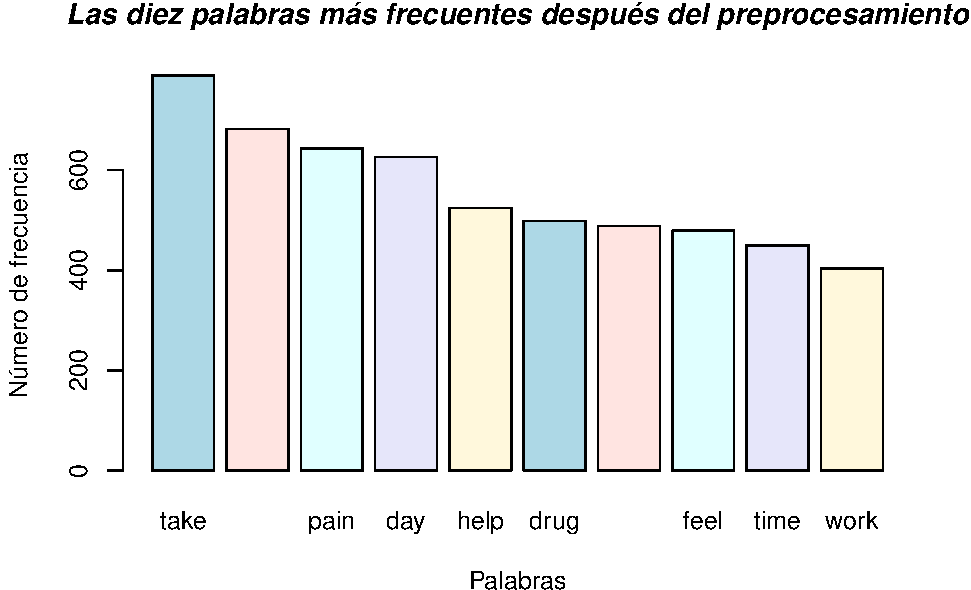
\includegraphics{practica_files/figure-latex/unnamed-chunk-38-1.pdf}


\end{document}
